\documentclass[leqno, 12pt]{article}
\usepackage{tikz}
\usetikzlibrary{positioning}
\usetikzlibrary {arrows.meta}
\usetikzlibrary{bending}
\usepackage{ulem}
\usepackage[a4paper, portrait, margin=1cm]{geometry}
\usepackage{fancyhdr}

\def\jumpheight{12}
\def\jumpheighthigh{18}
% \def\qgap{\rule[-1pt]{1.0em}{.25pt}}
\def\qgap{\raisebox{-1pt}{\dotuline{\phantom{X}}}}

\def \HeadingQuestions {\section*{\Large Name: \underline{\hspace{8cm}} \hfill Date: \underline{\hspace{3cm}}} \vspace{-3mm}
{<<title>>: Questions} \vspace{1pt}\hrule}

% raise footer with page number; no header
\fancypagestyle{myfancypagestyle}{
  \fancyhf{} % clear all header and footer fields
  \renewcommand{\headrulewidth}{0pt} % no rule under header
  \fancyfoot[C] {\thepage} \setlength{\footskip}{14.5pt} % raise page number 6pt
}
\pagestyle{myfancypagestyle}  % apply myfancypagestyle

\begin{document}
  \HeadingQuestions
  \vspace{-1mm}
  \begin{equation}
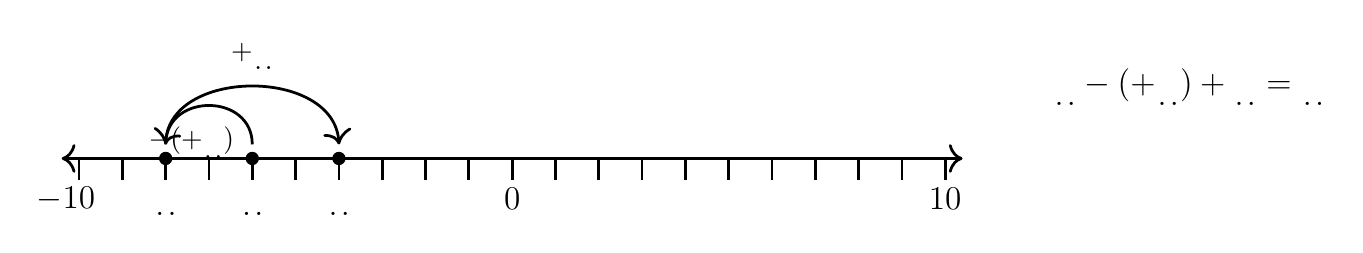
\begin{tikzpicture}[scale=0.55, baseline={([yshift=-1pt]current bounding box.north)}]
    % axis, arrow style to-to
    \draw[{To[scale=1.3]}-{To[scale=1.3]}, line width=1pt] (-10.4, 0) -- (10.4, 0);
    % tick marks
    \foreach \x in {-10,-9,...,10}
        \draw[shift={(\x,0)},color=black, line width=1pt] (0pt,-14pt) -- (0pt,0pt);
    % numbers along each axis
    \foreach \x in {-10}
        \draw[shift={(\x -0.3,-0.8)},color=black] node[font=\large,text height=12pt] {$\x$};
    \foreach \x in {0,10}
        \draw[shift={(\x,-0.8)},color=black] node[font=\large,text height=12pt] {$\x$};
    % numbers for dots
    \draw[shift={(-6,-0.8)},color=black] node[font=\large,text height=12pt] {$\qgap$};
    \draw[shift={(-8,-0.8)},color=black] node[font=\large,text height=12pt] {$\qgap$};
    \draw[shift={(-4,-0.8)},color=black] node[font=\large,text height=12pt] {$\qgap$};
    % dots
    \filldraw[black] (-6,0) circle (4pt) node[above,yshift=-2pt] (a) {};
    \filldraw[black] (-8,0) circle (4pt) node[above,yshift=-2pt] (m) {};
    \filldraw[black] (-4,0) circle (4pt) node[above,yshift=-2pt] (b) {};

    % first arrow (label below to left)
    \draw[-{To[scale=1.3, bend]}, line width=1pt, color=black] (a.north)
        .. controls +(north:\jumpheight mm) and +(north:\jumpheight mm) ..
        node[above=-9pt, xshift=-22pt, font=\normalsize, text height=8pt, pos=0] {$-(+\qgap)$} (m.north);

    % second arrow (label above)
    \draw[-{To[scale=1.3, bend]}, line width=1pt, color=black] (m.north)
        .. controls +(north:\jumpheighthigh mm) and +(north:\jumpheighthigh mm) ..
        node[above=2pt, font=\normalsize, text height=8pt] {$+\qgap$} (b.north);

    % equation at right end
    \node [font=\large, anchor=east] at (19,1.65) {$\qgap-(+\qgap)+\qgap = \qgap$};
\end{tikzpicture}
\end{equation}
\vspace{-2pt}\begin{equation}
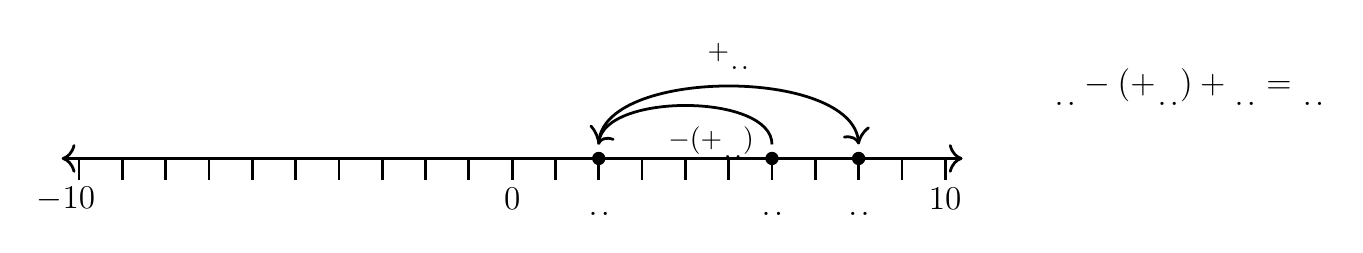
\begin{tikzpicture}[scale=0.55, baseline={([yshift=-1pt]current bounding box.north)}]
    % axis, arrow style to-to
    \draw[{To[scale=1.3]}-{To[scale=1.3]}, line width=1pt] (-10.4, 0) -- (10.4, 0);
    % tick marks
    \foreach \x in {-10,-9,...,10}
        \draw[shift={(\x,0)},color=black, line width=1pt] (0pt,-14pt) -- (0pt,0pt);
    % numbers along each axis
    \foreach \x in {-10}
        \draw[shift={(\x -0.3,-0.8)},color=black] node[font=\large,text height=12pt] {$\x$};
    \foreach \x in {0,10}
        \draw[shift={(\x,-0.8)},color=black] node[font=\large,text height=12pt] {$\x$};
    % numbers for dots
    \draw[shift={(6,-0.8)},color=black] node[font=\large,text height=12pt] {$\qgap$};
    \draw[shift={(2,-0.8)},color=black] node[font=\large,text height=12pt] {$\qgap$};
    \draw[shift={(8,-0.8)},color=black] node[font=\large,text height=12pt] {$\qgap$};
    % dots
    \filldraw[black] (6,0) circle (4pt) node[above,yshift=-2pt] (a) {};
    \filldraw[black] (2,0) circle (4pt) node[above,yshift=-2pt] (m) {};
    \filldraw[black] (8,0) circle (4pt) node[above,yshift=-2pt] (b) {};

    % first arrow (label below to left)
    \draw[-{To[scale=1.3, bend]}, line width=1pt, color=black] (a.north)
        .. controls +(north:\jumpheight mm) and +(north:\jumpheight mm) ..
        node[above=-9pt, xshift=-22pt, font=\normalsize, text height=8pt, pos=0] {$-(+\qgap)$} (m.north);

    % second arrow (label above)
    \draw[-{To[scale=1.3, bend]}, line width=1pt, color=black] (m.north)
        .. controls +(north:\jumpheighthigh mm) and +(north:\jumpheighthigh mm) ..
        node[above=2pt, font=\normalsize, text height=8pt] {$+\qgap$} (b.north);

    % equation at right end
    \node [font=\large, anchor=east] at (19,1.65) {$\qgap-(+\qgap)+\qgap = \qgap$};
\end{tikzpicture}
\end{equation}
\vspace{-2pt}\begin{equation}
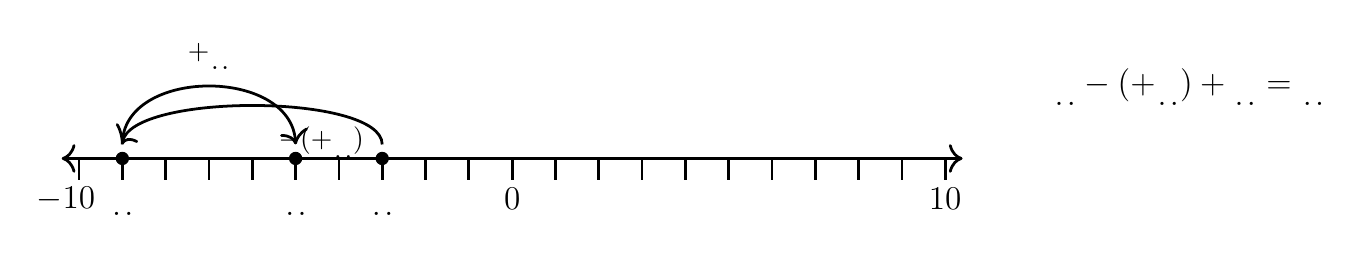
\begin{tikzpicture}[scale=0.55, baseline={([yshift=-1pt]current bounding box.north)}]
    % axis, arrow style to-to
    \draw[{To[scale=1.3]}-{To[scale=1.3]}, line width=1pt] (-10.4, 0) -- (10.4, 0);
    % tick marks
    \foreach \x in {-10,-9,...,10}
        \draw[shift={(\x,0)},color=black, line width=1pt] (0pt,-14pt) -- (0pt,0pt);
    % numbers along each axis
    \foreach \x in {-10}
        \draw[shift={(\x -0.3,-0.8)},color=black] node[font=\large,text height=12pt] {$\x$};
    \foreach \x in {0,10}
        \draw[shift={(\x,-0.8)},color=black] node[font=\large,text height=12pt] {$\x$};
    % numbers for dots
    \draw[shift={(-3,-0.8)},color=black] node[font=\large,text height=12pt] {$\qgap$};
    \draw[shift={(-9,-0.8)},color=black] node[font=\large,text height=12pt] {$\qgap$};
    \draw[shift={(-5,-0.8)},color=black] node[font=\large,text height=12pt] {$\qgap$};
    % dots
    \filldraw[black] (-3,0) circle (4pt) node[above,yshift=-2pt] (a) {};
    \filldraw[black] (-9,0) circle (4pt) node[above,yshift=-2pt] (m) {};
    \filldraw[black] (-5,0) circle (4pt) node[above,yshift=-2pt] (b) {};

    % first arrow (label below to left)
    \draw[-{To[scale=1.3, bend]}, line width=1pt, color=black] (a.north)
        .. controls +(north:\jumpheight mm) and +(north:\jumpheight mm) ..
        node[above=-9pt, xshift=-22pt, font=\normalsize, text height=8pt, pos=0] {$-(+\qgap)$} (m.north);

    % second arrow (label above)
    \draw[-{To[scale=1.3, bend]}, line width=1pt, color=black] (m.north)
        .. controls +(north:\jumpheighthigh mm) and +(north:\jumpheighthigh mm) ..
        node[above=2pt, font=\normalsize, text height=8pt] {$+\qgap$} (b.north);

    % equation at right end
    \node [font=\large, anchor=east] at (19,1.65) {$\qgap-(+\qgap)+\qgap = \qgap$};
\end{tikzpicture}
\end{equation}
\vspace{-2pt}\begin{equation}
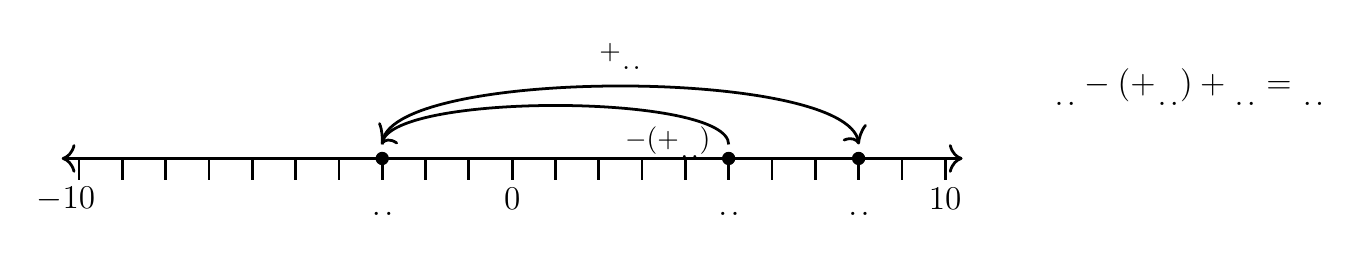
\begin{tikzpicture}[scale=0.55, baseline={([yshift=-1pt]current bounding box.north)}]
    % axis, arrow style to-to
    \draw[{To[scale=1.3]}-{To[scale=1.3]}, line width=1pt] (-10.4, 0) -- (10.4, 0);
    % tick marks
    \foreach \x in {-10,-9,...,10}
        \draw[shift={(\x,0)},color=black, line width=1pt] (0pt,-14pt) -- (0pt,0pt);
    % numbers along each axis
    \foreach \x in {-10}
        \draw[shift={(\x -0.3,-0.8)},color=black] node[font=\large,text height=12pt] {$\x$};
    \foreach \x in {0,10}
        \draw[shift={(\x,-0.8)},color=black] node[font=\large,text height=12pt] {$\x$};
    % numbers for dots
    \draw[shift={(5,-0.8)},color=black] node[font=\large,text height=12pt] {$\qgap$};
    \draw[shift={(-3,-0.8)},color=black] node[font=\large,text height=12pt] {$\qgap$};
    \draw[shift={(8,-0.8)},color=black] node[font=\large,text height=12pt] {$\qgap$};
    % dots
    \filldraw[black] (5,0) circle (4pt) node[above,yshift=-2pt] (a) {};
    \filldraw[black] (-3,0) circle (4pt) node[above,yshift=-2pt] (m) {};
    \filldraw[black] (8,0) circle (4pt) node[above,yshift=-2pt] (b) {};

    % first arrow (label below to left)
    \draw[-{To[scale=1.3, bend]}, line width=1pt, color=black] (a.north)
        .. controls +(north:\jumpheight mm) and +(north:\jumpheight mm) ..
        node[above=-9pt, xshift=-22pt, font=\normalsize, text height=8pt, pos=0] {$-(+\qgap)$} (m.north);

    % second arrow (label above)
    \draw[-{To[scale=1.3, bend]}, line width=1pt, color=black] (m.north)
        .. controls +(north:\jumpheighthigh mm) and +(north:\jumpheighthigh mm) ..
        node[above=2pt, font=\normalsize, text height=8pt] {$+\qgap$} (b.north);

    % equation at right end
    \node [font=\large, anchor=east] at (19,1.65) {$\qgap-(+\qgap)+\qgap = \qgap$};
\end{tikzpicture}
\end{equation}
\vspace{-2pt}\begin{equation}
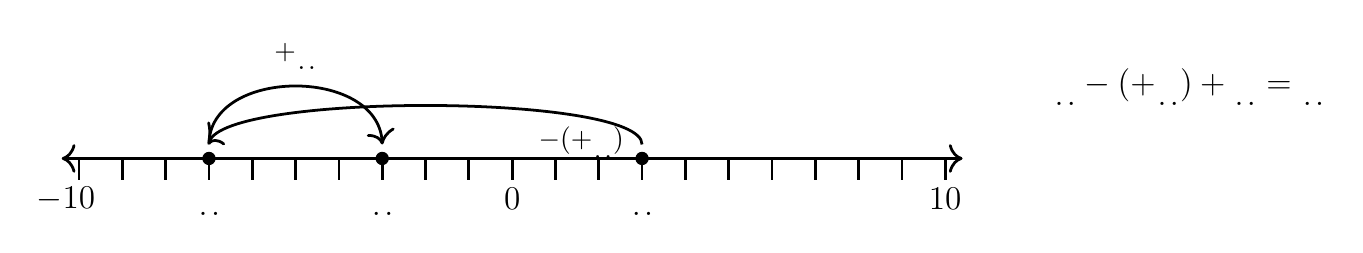
\begin{tikzpicture}[scale=0.55, baseline={([yshift=-1pt]current bounding box.north)}]
    % axis, arrow style to-to
    \draw[{To[scale=1.3]}-{To[scale=1.3]}, line width=1pt] (-10.4, 0) -- (10.4, 0);
    % tick marks
    \foreach \x in {-10,-9,...,10}
        \draw[shift={(\x,0)},color=black, line width=1pt] (0pt,-14pt) -- (0pt,0pt);
    % numbers along each axis
    \foreach \x in {-10}
        \draw[shift={(\x -0.3,-0.8)},color=black] node[font=\large,text height=12pt] {$\x$};
    \foreach \x in {0,10}
        \draw[shift={(\x,-0.8)},color=black] node[font=\large,text height=12pt] {$\x$};
    % numbers for dots
    \draw[shift={(3,-0.8)},color=black] node[font=\large,text height=12pt] {$\qgap$};
    \draw[shift={(-7,-0.8)},color=black] node[font=\large,text height=12pt] {$\qgap$};
    \draw[shift={(-3,-0.8)},color=black] node[font=\large,text height=12pt] {$\qgap$};
    % dots
    \filldraw[black] (3,0) circle (4pt) node[above,yshift=-2pt] (a) {};
    \filldraw[black] (-7,0) circle (4pt) node[above,yshift=-2pt] (m) {};
    \filldraw[black] (-3,0) circle (4pt) node[above,yshift=-2pt] (b) {};

    % first arrow (label below to left)
    \draw[-{To[scale=1.3, bend]}, line width=1pt, color=black] (a.north)
        .. controls +(north:\jumpheight mm) and +(north:\jumpheight mm) ..
        node[above=-9pt, xshift=-22pt, font=\normalsize, text height=8pt, pos=0] {$-(+\qgap)$} (m.north);

    % second arrow (label above)
    \draw[-{To[scale=1.3, bend]}, line width=1pt, color=black] (m.north)
        .. controls +(north:\jumpheighthigh mm) and +(north:\jumpheighthigh mm) ..
        node[above=2pt, font=\normalsize, text height=8pt] {$+\qgap$} (b.north);

    % equation at right end
    \node [font=\large, anchor=east] at (19,1.65) {$\qgap-(+\qgap)+\qgap = \qgap$};
\end{tikzpicture}
\end{equation}
\vspace{-2pt}\begin{equation}
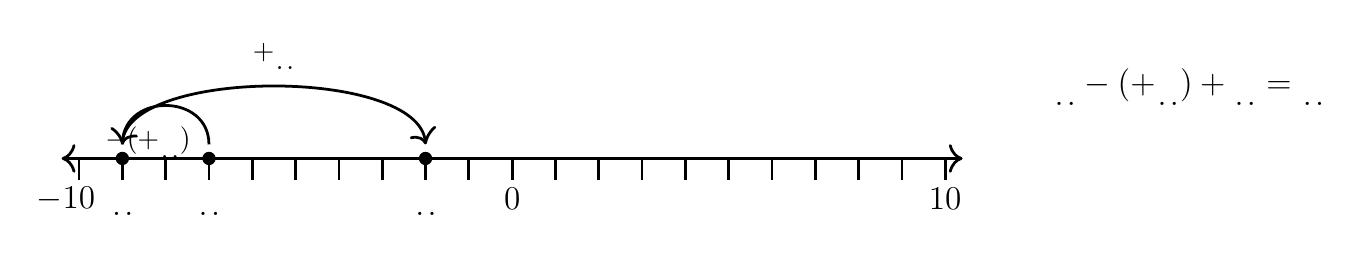
\begin{tikzpicture}[scale=0.55, baseline={([yshift=-1pt]current bounding box.north)}]
    % axis, arrow style to-to
    \draw[{To[scale=1.3]}-{To[scale=1.3]}, line width=1pt] (-10.4, 0) -- (10.4, 0);
    % tick marks
    \foreach \x in {-10,-9,...,10}
        \draw[shift={(\x,0)},color=black, line width=1pt] (0pt,-14pt) -- (0pt,0pt);
    % numbers along each axis
    \foreach \x in {-10}
        \draw[shift={(\x -0.3,-0.8)},color=black] node[font=\large,text height=12pt] {$\x$};
    \foreach \x in {0,10}
        \draw[shift={(\x,-0.8)},color=black] node[font=\large,text height=12pt] {$\x$};
    % numbers for dots
    \draw[shift={(-7,-0.8)},color=black] node[font=\large,text height=12pt] {$\qgap$};
    \draw[shift={(-9,-0.8)},color=black] node[font=\large,text height=12pt] {$\qgap$};
    \draw[shift={(-2,-0.8)},color=black] node[font=\large,text height=12pt] {$\qgap$};
    % dots
    \filldraw[black] (-7,0) circle (4pt) node[above,yshift=-2pt] (a) {};
    \filldraw[black] (-9,0) circle (4pt) node[above,yshift=-2pt] (m) {};
    \filldraw[black] (-2,0) circle (4pt) node[above,yshift=-2pt] (b) {};

    % first arrow (label below to left)
    \draw[-{To[scale=1.3, bend]}, line width=1pt, color=black] (a.north)
        .. controls +(north:\jumpheight mm) and +(north:\jumpheight mm) ..
        node[above=-9pt, xshift=-22pt, font=\normalsize, text height=8pt, pos=0] {$-(+\qgap)$} (m.north);

    % second arrow (label above)
    \draw[-{To[scale=1.3, bend]}, line width=1pt, color=black] (m.north)
        .. controls +(north:\jumpheighthigh mm) and +(north:\jumpheighthigh mm) ..
        node[above=2pt, font=\normalsize, text height=8pt] {$+\qgap$} (b.north);

    % equation at right end
    \node [font=\large, anchor=east] at (19,1.65) {$\qgap-(+\qgap)+\qgap = \qgap$};
\end{tikzpicture}
\end{equation}
\vspace{-2pt}\begin{equation}
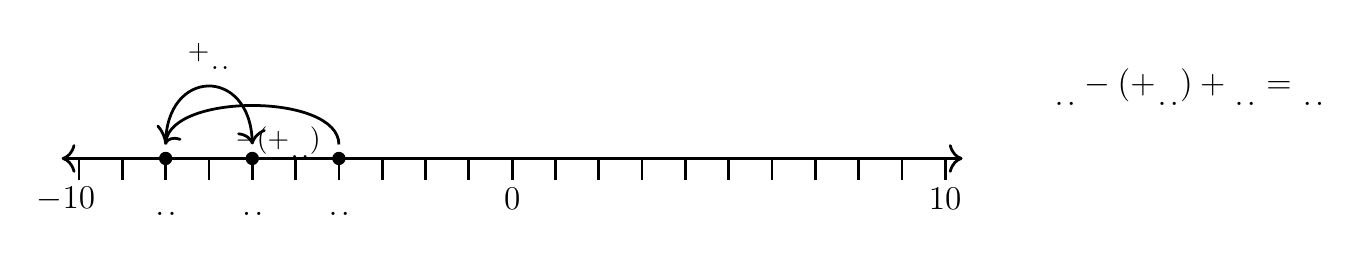
\begin{tikzpicture}[scale=0.55, baseline={([yshift=-1pt]current bounding box.north)}]
    % axis, arrow style to-to
    \draw[{To[scale=1.3]}-{To[scale=1.3]}, line width=1pt] (-10.4, 0) -- (10.4, 0);
    % tick marks
    \foreach \x in {-10,-9,...,10}
        \draw[shift={(\x,0)},color=black, line width=1pt] (0pt,-14pt) -- (0pt,0pt);
    % numbers along each axis
    \foreach \x in {-10}
        \draw[shift={(\x -0.3,-0.8)},color=black] node[font=\large,text height=12pt] {$\x$};
    \foreach \x in {0,10}
        \draw[shift={(\x,-0.8)},color=black] node[font=\large,text height=12pt] {$\x$};
    % numbers for dots
    \draw[shift={(-4,-0.8)},color=black] node[font=\large,text height=12pt] {$\qgap$};
    \draw[shift={(-8,-0.8)},color=black] node[font=\large,text height=12pt] {$\qgap$};
    \draw[shift={(-6,-0.8)},color=black] node[font=\large,text height=12pt] {$\qgap$};
    % dots
    \filldraw[black] (-4,0) circle (4pt) node[above,yshift=-2pt] (a) {};
    \filldraw[black] (-8,0) circle (4pt) node[above,yshift=-2pt] (m) {};
    \filldraw[black] (-6,0) circle (4pt) node[above,yshift=-2pt] (b) {};

    % first arrow (label below to left)
    \draw[-{To[scale=1.3, bend]}, line width=1pt, color=black] (a.north)
        .. controls +(north:\jumpheight mm) and +(north:\jumpheight mm) ..
        node[above=-9pt, xshift=-22pt, font=\normalsize, text height=8pt, pos=0] {$-(+\qgap)$} (m.north);

    % second arrow (label above)
    \draw[-{To[scale=1.3, bend]}, line width=1pt, color=black] (m.north)
        .. controls +(north:\jumpheighthigh mm) and +(north:\jumpheighthigh mm) ..
        node[above=2pt, font=\normalsize, text height=8pt] {$+\qgap$} (b.north);

    % equation at right end
    \node [font=\large, anchor=east] at (19,1.65) {$\qgap-(+\qgap)+\qgap = \qgap$};
\end{tikzpicture}
\end{equation}
\vspace{-2pt}\begin{equation}
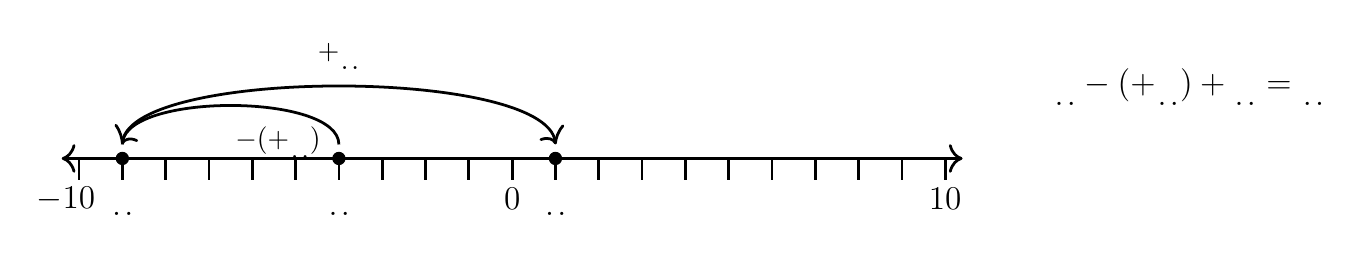
\begin{tikzpicture}[scale=0.55, baseline={([yshift=-1pt]current bounding box.north)}]
    % axis, arrow style to-to
    \draw[{To[scale=1.3]}-{To[scale=1.3]}, line width=1pt] (-10.4, 0) -- (10.4, 0);
    % tick marks
    \foreach \x in {-10,-9,...,10}
        \draw[shift={(\x,0)},color=black, line width=1pt] (0pt,-14pt) -- (0pt,0pt);
    % numbers along each axis
    \foreach \x in {-10}
        \draw[shift={(\x -0.3,-0.8)},color=black] node[font=\large,text height=12pt] {$\x$};
    \foreach \x in {0,10}
        \draw[shift={(\x,-0.8)},color=black] node[font=\large,text height=12pt] {$\x$};
    % numbers for dots
    \draw[shift={(-4,-0.8)},color=black] node[font=\large,text height=12pt] {$\qgap$};
    \draw[shift={(-9,-0.8)},color=black] node[font=\large,text height=12pt] {$\qgap$};
    \draw[shift={(1,-0.8)},color=black] node[font=\large,text height=12pt] {$\qgap$};
    % dots
    \filldraw[black] (-4,0) circle (4pt) node[above,yshift=-2pt] (a) {};
    \filldraw[black] (-9,0) circle (4pt) node[above,yshift=-2pt] (m) {};
    \filldraw[black] (1,0) circle (4pt) node[above,yshift=-2pt] (b) {};

    % first arrow (label below to left)
    \draw[-{To[scale=1.3, bend]}, line width=1pt, color=black] (a.north)
        .. controls +(north:\jumpheight mm) and +(north:\jumpheight mm) ..
        node[above=-9pt, xshift=-22pt, font=\normalsize, text height=8pt, pos=0] {$-(+\qgap)$} (m.north);

    % second arrow (label above)
    \draw[-{To[scale=1.3, bend]}, line width=1pt, color=black] (m.north)
        .. controls +(north:\jumpheighthigh mm) and +(north:\jumpheighthigh mm) ..
        node[above=2pt, font=\normalsize, text height=8pt] {$+\qgap$} (b.north);

    % equation at right end
    \node [font=\large, anchor=east] at (19,1.65) {$\qgap-(+\qgap)+\qgap = \qgap$};
\end{tikzpicture}
\end{equation}
\vspace{-2pt}\pagebreak ~ \newline ~ \newline\begin{equation}
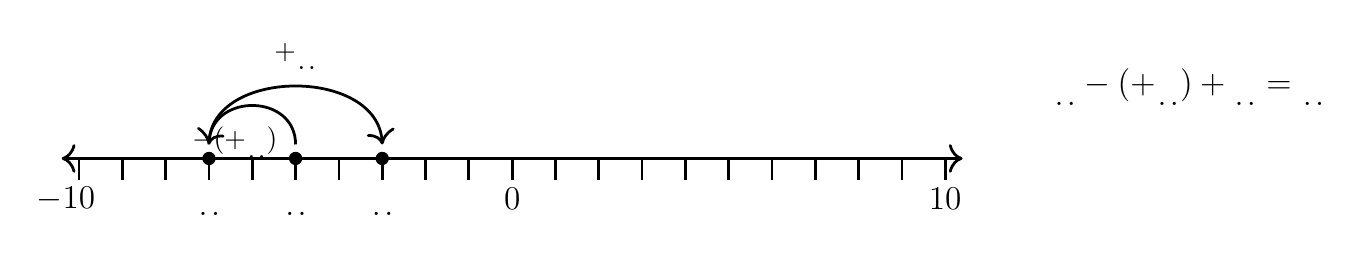
\begin{tikzpicture}[scale=0.55, baseline={([yshift=-1pt]current bounding box.north)}]
    % axis, arrow style to-to
    \draw[{To[scale=1.3]}-{To[scale=1.3]}, line width=1pt] (-10.4, 0) -- (10.4, 0);
    % tick marks
    \foreach \x in {-10,-9,...,10}
        \draw[shift={(\x,0)},color=black, line width=1pt] (0pt,-14pt) -- (0pt,0pt);
    % numbers along each axis
    \foreach \x in {-10}
        \draw[shift={(\x -0.3,-0.8)},color=black] node[font=\large,text height=12pt] {$\x$};
    \foreach \x in {0,10}
        \draw[shift={(\x,-0.8)},color=black] node[font=\large,text height=12pt] {$\x$};
    % numbers for dots
    \draw[shift={(-5,-0.8)},color=black] node[font=\large,text height=12pt] {$\qgap$};
    \draw[shift={(-7,-0.8)},color=black] node[font=\large,text height=12pt] {$\qgap$};
    \draw[shift={(-3,-0.8)},color=black] node[font=\large,text height=12pt] {$\qgap$};
    % dots
    \filldraw[black] (-5,0) circle (4pt) node[above,yshift=-2pt] (a) {};
    \filldraw[black] (-7,0) circle (4pt) node[above,yshift=-2pt] (m) {};
    \filldraw[black] (-3,0) circle (4pt) node[above,yshift=-2pt] (b) {};

    % first arrow (label below to left)
    \draw[-{To[scale=1.3, bend]}, line width=1pt, color=black] (a.north)
        .. controls +(north:\jumpheight mm) and +(north:\jumpheight mm) ..
        node[above=-9pt, xshift=-22pt, font=\normalsize, text height=8pt, pos=0] {$-(+\qgap)$} (m.north);

    % second arrow (label above)
    \draw[-{To[scale=1.3, bend]}, line width=1pt, color=black] (m.north)
        .. controls +(north:\jumpheighthigh mm) and +(north:\jumpheighthigh mm) ..
        node[above=2pt, font=\normalsize, text height=8pt] {$+\qgap$} (b.north);

    % equation at right end
    \node [font=\large, anchor=east] at (19,1.65) {$\qgap-(+\qgap)+\qgap = \qgap$};
\end{tikzpicture}
\end{equation}
\vspace{-2pt}\begin{equation}
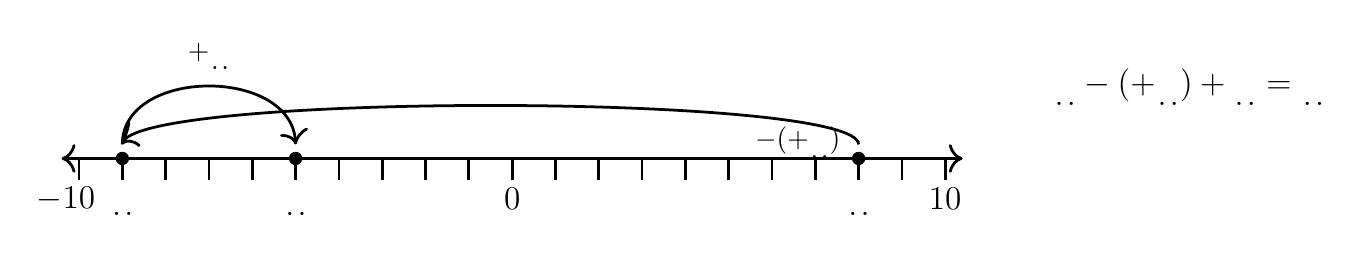
\begin{tikzpicture}[scale=0.55, baseline={([yshift=-1pt]current bounding box.north)}]
    % axis, arrow style to-to
    \draw[{To[scale=1.3]}-{To[scale=1.3]}, line width=1pt] (-10.4, 0) -- (10.4, 0);
    % tick marks
    \foreach \x in {-10,-9,...,10}
        \draw[shift={(\x,0)},color=black, line width=1pt] (0pt,-14pt) -- (0pt,0pt);
    % numbers along each axis
    \foreach \x in {-10}
        \draw[shift={(\x -0.3,-0.8)},color=black] node[font=\large,text height=12pt] {$\x$};
    \foreach \x in {0,10}
        \draw[shift={(\x,-0.8)},color=black] node[font=\large,text height=12pt] {$\x$};
    % numbers for dots
    \draw[shift={(8,-0.8)},color=black] node[font=\large,text height=12pt] {$\qgap$};
    \draw[shift={(-9,-0.8)},color=black] node[font=\large,text height=12pt] {$\qgap$};
    \draw[shift={(-5,-0.8)},color=black] node[font=\large,text height=12pt] {$\qgap$};
    % dots
    \filldraw[black] (8,0) circle (4pt) node[above,yshift=-2pt] (a) {};
    \filldraw[black] (-9,0) circle (4pt) node[above,yshift=-2pt] (m) {};
    \filldraw[black] (-5,0) circle (4pt) node[above,yshift=-2pt] (b) {};

    % first arrow (label below to left)
    \draw[-{To[scale=1.3, bend]}, line width=1pt, color=black] (a.north)
        .. controls +(north:\jumpheight mm) and +(north:\jumpheight mm) ..
        node[above=-9pt, xshift=-22pt, font=\normalsize, text height=8pt, pos=0] {$-(+\qgap)$} (m.north);

    % second arrow (label above)
    \draw[-{To[scale=1.3, bend]}, line width=1pt, color=black] (m.north)
        .. controls +(north:\jumpheighthigh mm) and +(north:\jumpheighthigh mm) ..
        node[above=2pt, font=\normalsize, text height=8pt] {$+\qgap$} (b.north);

    % equation at right end
    \node [font=\large, anchor=east] at (19,1.65) {$\qgap-(+\qgap)+\qgap = \qgap$};
\end{tikzpicture}
\end{equation}
\vspace{-2pt}\begin{equation}
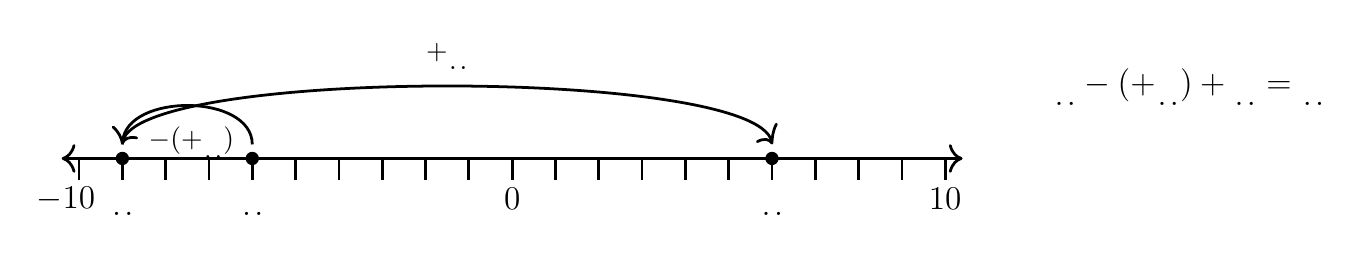
\begin{tikzpicture}[scale=0.55, baseline={([yshift=-1pt]current bounding box.north)}]
    % axis, arrow style to-to
    \draw[{To[scale=1.3]}-{To[scale=1.3]}, line width=1pt] (-10.4, 0) -- (10.4, 0);
    % tick marks
    \foreach \x in {-10,-9,...,10}
        \draw[shift={(\x,0)},color=black, line width=1pt] (0pt,-14pt) -- (0pt,0pt);
    % numbers along each axis
    \foreach \x in {-10}
        \draw[shift={(\x -0.3,-0.8)},color=black] node[font=\large,text height=12pt] {$\x$};
    \foreach \x in {0,10}
        \draw[shift={(\x,-0.8)},color=black] node[font=\large,text height=12pt] {$\x$};
    % numbers for dots
    \draw[shift={(-6,-0.8)},color=black] node[font=\large,text height=12pt] {$\qgap$};
    \draw[shift={(-9,-0.8)},color=black] node[font=\large,text height=12pt] {$\qgap$};
    \draw[shift={(6,-0.8)},color=black] node[font=\large,text height=12pt] {$\qgap$};
    % dots
    \filldraw[black] (-6,0) circle (4pt) node[above,yshift=-2pt] (a) {};
    \filldraw[black] (-9,0) circle (4pt) node[above,yshift=-2pt] (m) {};
    \filldraw[black] (6,0) circle (4pt) node[above,yshift=-2pt] (b) {};

    % first arrow (label below to left)
    \draw[-{To[scale=1.3, bend]}, line width=1pt, color=black] (a.north)
        .. controls +(north:\jumpheight mm) and +(north:\jumpheight mm) ..
        node[above=-9pt, xshift=-22pt, font=\normalsize, text height=8pt, pos=0] {$-(+\qgap)$} (m.north);

    % second arrow (label above)
    \draw[-{To[scale=1.3, bend]}, line width=1pt, color=black] (m.north)
        .. controls +(north:\jumpheighthigh mm) and +(north:\jumpheighthigh mm) ..
        node[above=2pt, font=\normalsize, text height=8pt] {$+\qgap$} (b.north);

    % equation at right end
    \node [font=\large, anchor=east] at (19,1.65) {$\qgap-(+\qgap)+\qgap = \qgap$};
\end{tikzpicture}
\end{equation}
\vspace{-2pt}\begin{equation}
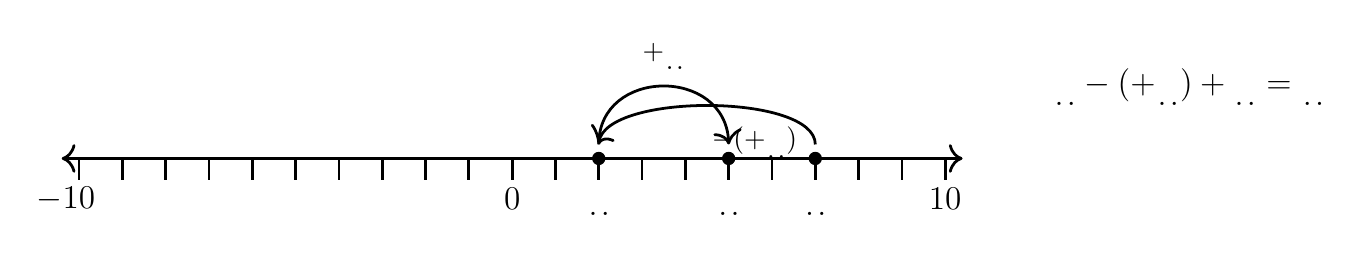
\begin{tikzpicture}[scale=0.55, baseline={([yshift=-1pt]current bounding box.north)}]
    % axis, arrow style to-to
    \draw[{To[scale=1.3]}-{To[scale=1.3]}, line width=1pt] (-10.4, 0) -- (10.4, 0);
    % tick marks
    \foreach \x in {-10,-9,...,10}
        \draw[shift={(\x,0)},color=black, line width=1pt] (0pt,-14pt) -- (0pt,0pt);
    % numbers along each axis
    \foreach \x in {-10}
        \draw[shift={(\x -0.3,-0.8)},color=black] node[font=\large,text height=12pt] {$\x$};
    \foreach \x in {0,10}
        \draw[shift={(\x,-0.8)},color=black] node[font=\large,text height=12pt] {$\x$};
    % numbers for dots
    \draw[shift={(7,-0.8)},color=black] node[font=\large,text height=12pt] {$\qgap$};
    \draw[shift={(2,-0.8)},color=black] node[font=\large,text height=12pt] {$\qgap$};
    \draw[shift={(5,-0.8)},color=black] node[font=\large,text height=12pt] {$\qgap$};
    % dots
    \filldraw[black] (7,0) circle (4pt) node[above,yshift=-2pt] (a) {};
    \filldraw[black] (2,0) circle (4pt) node[above,yshift=-2pt] (m) {};
    \filldraw[black] (5,0) circle (4pt) node[above,yshift=-2pt] (b) {};

    % first arrow (label below to left)
    \draw[-{To[scale=1.3, bend]}, line width=1pt, color=black] (a.north)
        .. controls +(north:\jumpheight mm) and +(north:\jumpheight mm) ..
        node[above=-9pt, xshift=-22pt, font=\normalsize, text height=8pt, pos=0] {$-(+\qgap)$} (m.north);

    % second arrow (label above)
    \draw[-{To[scale=1.3, bend]}, line width=1pt, color=black] (m.north)
        .. controls +(north:\jumpheighthigh mm) and +(north:\jumpheighthigh mm) ..
        node[above=2pt, font=\normalsize, text height=8pt] {$+\qgap$} (b.north);

    % equation at right end
    \node [font=\large, anchor=east] at (19,1.65) {$\qgap-(+\qgap)+\qgap = \qgap$};
\end{tikzpicture}
\end{equation}
\vspace{-2pt}\begin{equation}
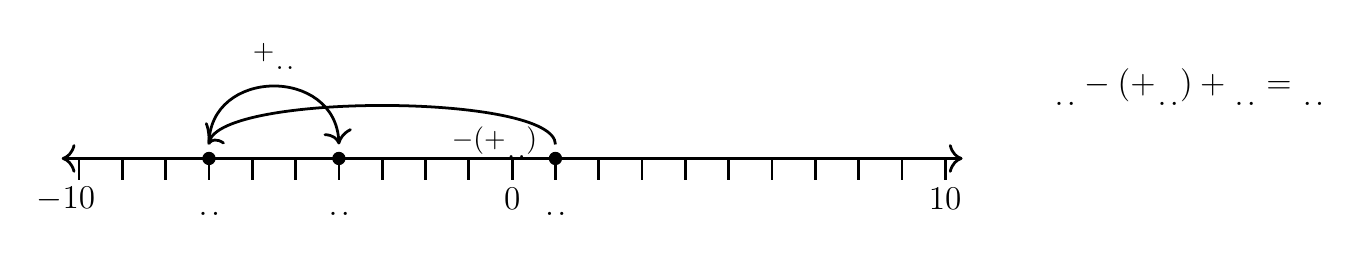
\begin{tikzpicture}[scale=0.55, baseline={([yshift=-1pt]current bounding box.north)}]
    % axis, arrow style to-to
    \draw[{To[scale=1.3]}-{To[scale=1.3]}, line width=1pt] (-10.4, 0) -- (10.4, 0);
    % tick marks
    \foreach \x in {-10,-9,...,10}
        \draw[shift={(\x,0)},color=black, line width=1pt] (0pt,-14pt) -- (0pt,0pt);
    % numbers along each axis
    \foreach \x in {-10}
        \draw[shift={(\x -0.3,-0.8)},color=black] node[font=\large,text height=12pt] {$\x$};
    \foreach \x in {0,10}
        \draw[shift={(\x,-0.8)},color=black] node[font=\large,text height=12pt] {$\x$};
    % numbers for dots
    \draw[shift={(1,-0.8)},color=black] node[font=\large,text height=12pt] {$\qgap$};
    \draw[shift={(-7,-0.8)},color=black] node[font=\large,text height=12pt] {$\qgap$};
    \draw[shift={(-4,-0.8)},color=black] node[font=\large,text height=12pt] {$\qgap$};
    % dots
    \filldraw[black] (1,0) circle (4pt) node[above,yshift=-2pt] (a) {};
    \filldraw[black] (-7,0) circle (4pt) node[above,yshift=-2pt] (m) {};
    \filldraw[black] (-4,0) circle (4pt) node[above,yshift=-2pt] (b) {};

    % first arrow (label below to left)
    \draw[-{To[scale=1.3, bend]}, line width=1pt, color=black] (a.north)
        .. controls +(north:\jumpheight mm) and +(north:\jumpheight mm) ..
        node[above=-9pt, xshift=-22pt, font=\normalsize, text height=8pt, pos=0] {$-(+\qgap)$} (m.north);

    % second arrow (label above)
    \draw[-{To[scale=1.3, bend]}, line width=1pt, color=black] (m.north)
        .. controls +(north:\jumpheighthigh mm) and +(north:\jumpheighthigh mm) ..
        node[above=2pt, font=\normalsize, text height=8pt] {$+\qgap$} (b.north);

    % equation at right end
    \node [font=\large, anchor=east] at (19,1.65) {$\qgap-(+\qgap)+\qgap = \qgap$};
\end{tikzpicture}
\end{equation}
\vspace{-2pt}\begin{equation}
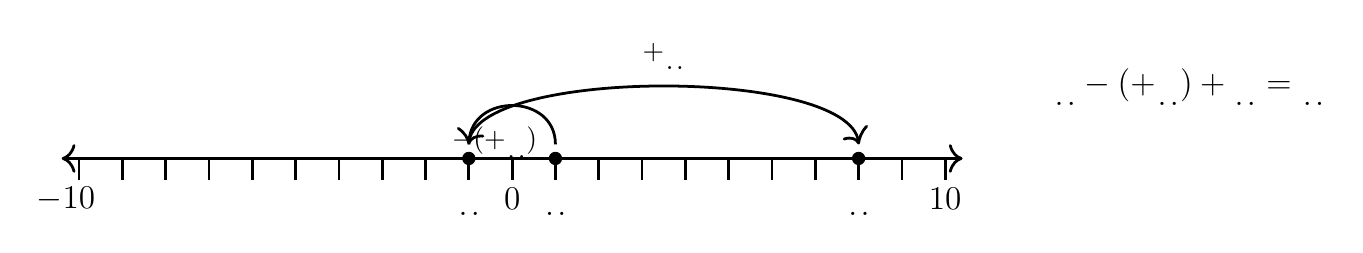
\begin{tikzpicture}[scale=0.55, baseline={([yshift=-1pt]current bounding box.north)}]
    % axis, arrow style to-to
    \draw[{To[scale=1.3]}-{To[scale=1.3]}, line width=1pt] (-10.4, 0) -- (10.4, 0);
    % tick marks
    \foreach \x in {-10,-9,...,10}
        \draw[shift={(\x,0)},color=black, line width=1pt] (0pt,-14pt) -- (0pt,0pt);
    % numbers along each axis
    \foreach \x in {-10}
        \draw[shift={(\x -0.3,-0.8)},color=black] node[font=\large,text height=12pt] {$\x$};
    \foreach \x in {0,10}
        \draw[shift={(\x,-0.8)},color=black] node[font=\large,text height=12pt] {$\x$};
    % numbers for dots
    \draw[shift={(1,-0.8)},color=black] node[font=\large,text height=12pt] {$\qgap$};
    \draw[shift={(-1,-0.8)},color=black] node[font=\large,text height=12pt] {$\qgap$};
    \draw[shift={(8,-0.8)},color=black] node[font=\large,text height=12pt] {$\qgap$};
    % dots
    \filldraw[black] (1,0) circle (4pt) node[above,yshift=-2pt] (a) {};
    \filldraw[black] (-1,0) circle (4pt) node[above,yshift=-2pt] (m) {};
    \filldraw[black] (8,0) circle (4pt) node[above,yshift=-2pt] (b) {};

    % first arrow (label below to left)
    \draw[-{To[scale=1.3, bend]}, line width=1pt, color=black] (a.north)
        .. controls +(north:\jumpheight mm) and +(north:\jumpheight mm) ..
        node[above=-9pt, xshift=-22pt, font=\normalsize, text height=8pt, pos=0] {$-(+\qgap)$} (m.north);

    % second arrow (label above)
    \draw[-{To[scale=1.3, bend]}, line width=1pt, color=black] (m.north)
        .. controls +(north:\jumpheighthigh mm) and +(north:\jumpheighthigh mm) ..
        node[above=2pt, font=\normalsize, text height=8pt] {$+\qgap$} (b.north);

    % equation at right end
    \node [font=\large, anchor=east] at (19,1.65) {$\qgap-(+\qgap)+\qgap = \qgap$};
\end{tikzpicture}
\end{equation}
\vspace{-2pt}\begin{equation}
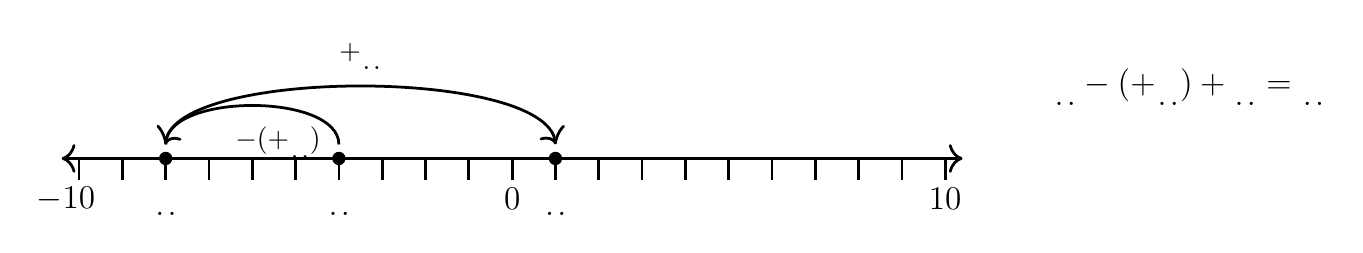
\begin{tikzpicture}[scale=0.55, baseline={([yshift=-1pt]current bounding box.north)}]
    % axis, arrow style to-to
    \draw[{To[scale=1.3]}-{To[scale=1.3]}, line width=1pt] (-10.4, 0) -- (10.4, 0);
    % tick marks
    \foreach \x in {-10,-9,...,10}
        \draw[shift={(\x,0)},color=black, line width=1pt] (0pt,-14pt) -- (0pt,0pt);
    % numbers along each axis
    \foreach \x in {-10}
        \draw[shift={(\x -0.3,-0.8)},color=black] node[font=\large,text height=12pt] {$\x$};
    \foreach \x in {0,10}
        \draw[shift={(\x,-0.8)},color=black] node[font=\large,text height=12pt] {$\x$};
    % numbers for dots
    \draw[shift={(-4,-0.8)},color=black] node[font=\large,text height=12pt] {$\qgap$};
    \draw[shift={(-8,-0.8)},color=black] node[font=\large,text height=12pt] {$\qgap$};
    \draw[shift={(1,-0.8)},color=black] node[font=\large,text height=12pt] {$\qgap$};
    % dots
    \filldraw[black] (-4,0) circle (4pt) node[above,yshift=-2pt] (a) {};
    \filldraw[black] (-8,0) circle (4pt) node[above,yshift=-2pt] (m) {};
    \filldraw[black] (1,0) circle (4pt) node[above,yshift=-2pt] (b) {};

    % first arrow (label below to left)
    \draw[-{To[scale=1.3, bend]}, line width=1pt, color=black] (a.north)
        .. controls +(north:\jumpheight mm) and +(north:\jumpheight mm) ..
        node[above=-9pt, xshift=-22pt, font=\normalsize, text height=8pt, pos=0] {$-(+\qgap)$} (m.north);

    % second arrow (label above)
    \draw[-{To[scale=1.3, bend]}, line width=1pt, color=black] (m.north)
        .. controls +(north:\jumpheighthigh mm) and +(north:\jumpheighthigh mm) ..
        node[above=2pt, font=\normalsize, text height=8pt] {$+\qgap$} (b.north);

    % equation at right end
    \node [font=\large, anchor=east] at (19,1.65) {$\qgap-(+\qgap)+\qgap = \qgap$};
\end{tikzpicture}
\end{equation}
\vspace{-2pt}\begin{equation}
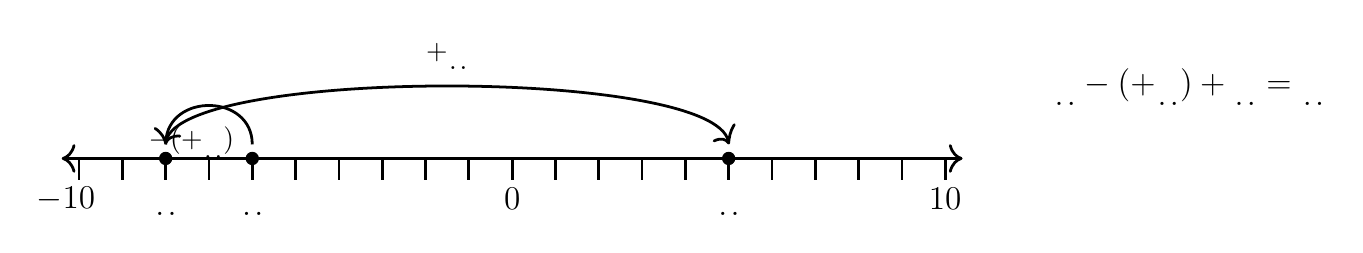
\begin{tikzpicture}[scale=0.55, baseline={([yshift=-1pt]current bounding box.north)}]
    % axis, arrow style to-to
    \draw[{To[scale=1.3]}-{To[scale=1.3]}, line width=1pt] (-10.4, 0) -- (10.4, 0);
    % tick marks
    \foreach \x in {-10,-9,...,10}
        \draw[shift={(\x,0)},color=black, line width=1pt] (0pt,-14pt) -- (0pt,0pt);
    % numbers along each axis
    \foreach \x in {-10}
        \draw[shift={(\x -0.3,-0.8)},color=black] node[font=\large,text height=12pt] {$\x$};
    \foreach \x in {0,10}
        \draw[shift={(\x,-0.8)},color=black] node[font=\large,text height=12pt] {$\x$};
    % numbers for dots
    \draw[shift={(-6,-0.8)},color=black] node[font=\large,text height=12pt] {$\qgap$};
    \draw[shift={(-8,-0.8)},color=black] node[font=\large,text height=12pt] {$\qgap$};
    \draw[shift={(5,-0.8)},color=black] node[font=\large,text height=12pt] {$\qgap$};
    % dots
    \filldraw[black] (-6,0) circle (4pt) node[above,yshift=-2pt] (a) {};
    \filldraw[black] (-8,0) circle (4pt) node[above,yshift=-2pt] (m) {};
    \filldraw[black] (5,0) circle (4pt) node[above,yshift=-2pt] (b) {};

    % first arrow (label below to left)
    \draw[-{To[scale=1.3, bend]}, line width=1pt, color=black] (a.north)
        .. controls +(north:\jumpheight mm) and +(north:\jumpheight mm) ..
        node[above=-9pt, xshift=-22pt, font=\normalsize, text height=8pt, pos=0] {$-(+\qgap)$} (m.north);

    % second arrow (label above)
    \draw[-{To[scale=1.3, bend]}, line width=1pt, color=black] (m.north)
        .. controls +(north:\jumpheighthigh mm) and +(north:\jumpheighthigh mm) ..
        node[above=2pt, font=\normalsize, text height=8pt] {$+\qgap$} (b.north);

    % equation at right end
    \node [font=\large, anchor=east] at (19,1.65) {$\qgap-(+\qgap)+\qgap = \qgap$};
\end{tikzpicture}
\end{equation}
\vspace{-2pt}\pagebreak ~ \newline ~ \newline\begin{equation}
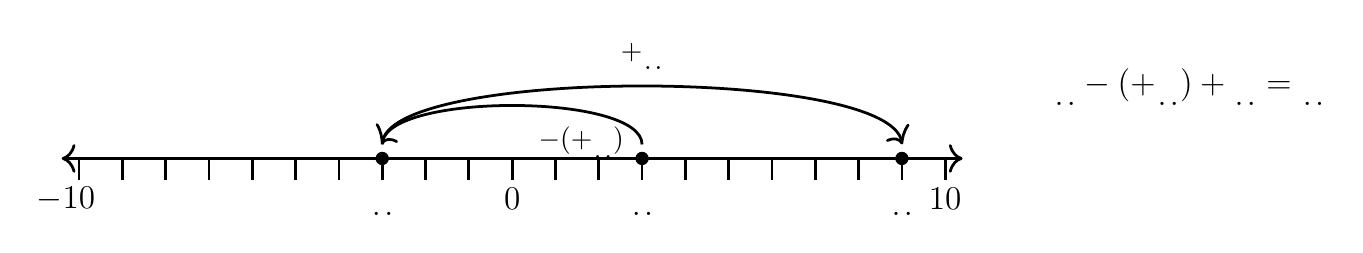
\begin{tikzpicture}[scale=0.55, baseline={([yshift=-1pt]current bounding box.north)}]
    % axis, arrow style to-to
    \draw[{To[scale=1.3]}-{To[scale=1.3]}, line width=1pt] (-10.4, 0) -- (10.4, 0);
    % tick marks
    \foreach \x in {-10,-9,...,10}
        \draw[shift={(\x,0)},color=black, line width=1pt] (0pt,-14pt) -- (0pt,0pt);
    % numbers along each axis
    \foreach \x in {-10}
        \draw[shift={(\x -0.3,-0.8)},color=black] node[font=\large,text height=12pt] {$\x$};
    \foreach \x in {0,10}
        \draw[shift={(\x,-0.8)},color=black] node[font=\large,text height=12pt] {$\x$};
    % numbers for dots
    \draw[shift={(3,-0.8)},color=black] node[font=\large,text height=12pt] {$\qgap$};
    \draw[shift={(-3,-0.8)},color=black] node[font=\large,text height=12pt] {$\qgap$};
    \draw[shift={(9,-0.8)},color=black] node[font=\large,text height=12pt] {$\qgap$};
    % dots
    \filldraw[black] (3,0) circle (4pt) node[above,yshift=-2pt] (a) {};
    \filldraw[black] (-3,0) circle (4pt) node[above,yshift=-2pt] (m) {};
    \filldraw[black] (9,0) circle (4pt) node[above,yshift=-2pt] (b) {};

    % first arrow (label below to left)
    \draw[-{To[scale=1.3, bend]}, line width=1pt, color=black] (a.north)
        .. controls +(north:\jumpheight mm) and +(north:\jumpheight mm) ..
        node[above=-9pt, xshift=-22pt, font=\normalsize, text height=8pt, pos=0] {$-(+\qgap)$} (m.north);

    % second arrow (label above)
    \draw[-{To[scale=1.3, bend]}, line width=1pt, color=black] (m.north)
        .. controls +(north:\jumpheighthigh mm) and +(north:\jumpheighthigh mm) ..
        node[above=2pt, font=\normalsize, text height=8pt] {$+\qgap$} (b.north);

    % equation at right end
    \node [font=\large, anchor=east] at (19,1.65) {$\qgap-(+\qgap)+\qgap = \qgap$};
\end{tikzpicture}
\end{equation}
\vspace{-2pt}\begin{equation}
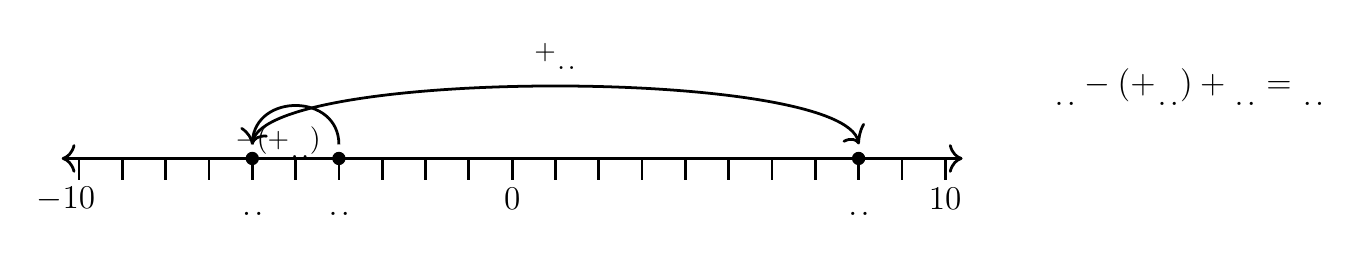
\begin{tikzpicture}[scale=0.55, baseline={([yshift=-1pt]current bounding box.north)}]
    % axis, arrow style to-to
    \draw[{To[scale=1.3]}-{To[scale=1.3]}, line width=1pt] (-10.4, 0) -- (10.4, 0);
    % tick marks
    \foreach \x in {-10,-9,...,10}
        \draw[shift={(\x,0)},color=black, line width=1pt] (0pt,-14pt) -- (0pt,0pt);
    % numbers along each axis
    \foreach \x in {-10}
        \draw[shift={(\x -0.3,-0.8)},color=black] node[font=\large,text height=12pt] {$\x$};
    \foreach \x in {0,10}
        \draw[shift={(\x,-0.8)},color=black] node[font=\large,text height=12pt] {$\x$};
    % numbers for dots
    \draw[shift={(-4,-0.8)},color=black] node[font=\large,text height=12pt] {$\qgap$};
    \draw[shift={(-6,-0.8)},color=black] node[font=\large,text height=12pt] {$\qgap$};
    \draw[shift={(8,-0.8)},color=black] node[font=\large,text height=12pt] {$\qgap$};
    % dots
    \filldraw[black] (-4,0) circle (4pt) node[above,yshift=-2pt] (a) {};
    \filldraw[black] (-6,0) circle (4pt) node[above,yshift=-2pt] (m) {};
    \filldraw[black] (8,0) circle (4pt) node[above,yshift=-2pt] (b) {};

    % first arrow (label below to left)
    \draw[-{To[scale=1.3, bend]}, line width=1pt, color=black] (a.north)
        .. controls +(north:\jumpheight mm) and +(north:\jumpheight mm) ..
        node[above=-9pt, xshift=-22pt, font=\normalsize, text height=8pt, pos=0] {$-(+\qgap)$} (m.north);

    % second arrow (label above)
    \draw[-{To[scale=1.3, bend]}, line width=1pt, color=black] (m.north)
        .. controls +(north:\jumpheighthigh mm) and +(north:\jumpheighthigh mm) ..
        node[above=2pt, font=\normalsize, text height=8pt] {$+\qgap$} (b.north);

    % equation at right end
    \node [font=\large, anchor=east] at (19,1.65) {$\qgap-(+\qgap)+\qgap = \qgap$};
\end{tikzpicture}
\end{equation}
\vspace{-2pt}\begin{equation}
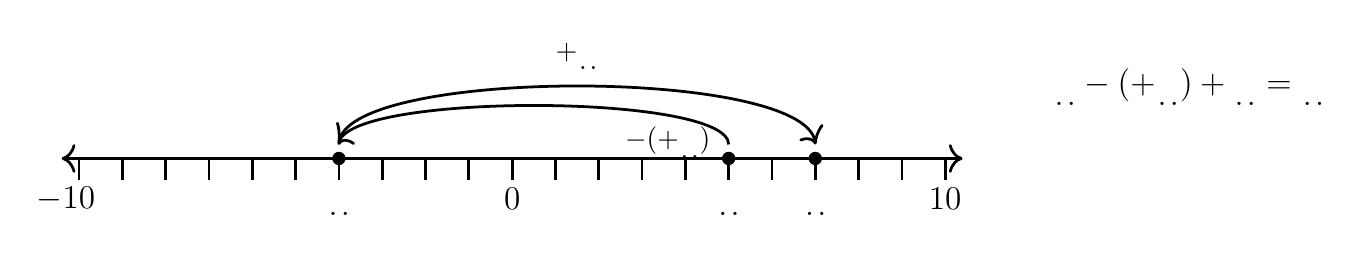
\begin{tikzpicture}[scale=0.55, baseline={([yshift=-1pt]current bounding box.north)}]
    % axis, arrow style to-to
    \draw[{To[scale=1.3]}-{To[scale=1.3]}, line width=1pt] (-10.4, 0) -- (10.4, 0);
    % tick marks
    \foreach \x in {-10,-9,...,10}
        \draw[shift={(\x,0)},color=black, line width=1pt] (0pt,-14pt) -- (0pt,0pt);
    % numbers along each axis
    \foreach \x in {-10}
        \draw[shift={(\x -0.3,-0.8)},color=black] node[font=\large,text height=12pt] {$\x$};
    \foreach \x in {0,10}
        \draw[shift={(\x,-0.8)},color=black] node[font=\large,text height=12pt] {$\x$};
    % numbers for dots
    \draw[shift={(5,-0.8)},color=black] node[font=\large,text height=12pt] {$\qgap$};
    \draw[shift={(-4,-0.8)},color=black] node[font=\large,text height=12pt] {$\qgap$};
    \draw[shift={(7,-0.8)},color=black] node[font=\large,text height=12pt] {$\qgap$};
    % dots
    \filldraw[black] (5,0) circle (4pt) node[above,yshift=-2pt] (a) {};
    \filldraw[black] (-4,0) circle (4pt) node[above,yshift=-2pt] (m) {};
    \filldraw[black] (7,0) circle (4pt) node[above,yshift=-2pt] (b) {};

    % first arrow (label below to left)
    \draw[-{To[scale=1.3, bend]}, line width=1pt, color=black] (a.north)
        .. controls +(north:\jumpheight mm) and +(north:\jumpheight mm) ..
        node[above=-9pt, xshift=-22pt, font=\normalsize, text height=8pt, pos=0] {$-(+\qgap)$} (m.north);

    % second arrow (label above)
    \draw[-{To[scale=1.3, bend]}, line width=1pt, color=black] (m.north)
        .. controls +(north:\jumpheighthigh mm) and +(north:\jumpheighthigh mm) ..
        node[above=2pt, font=\normalsize, text height=8pt] {$+\qgap$} (b.north);

    % equation at right end
    \node [font=\large, anchor=east] at (19,1.65) {$\qgap-(+\qgap)+\qgap = \qgap$};
\end{tikzpicture}
\end{equation}
\vspace{-2pt}\begin{equation}
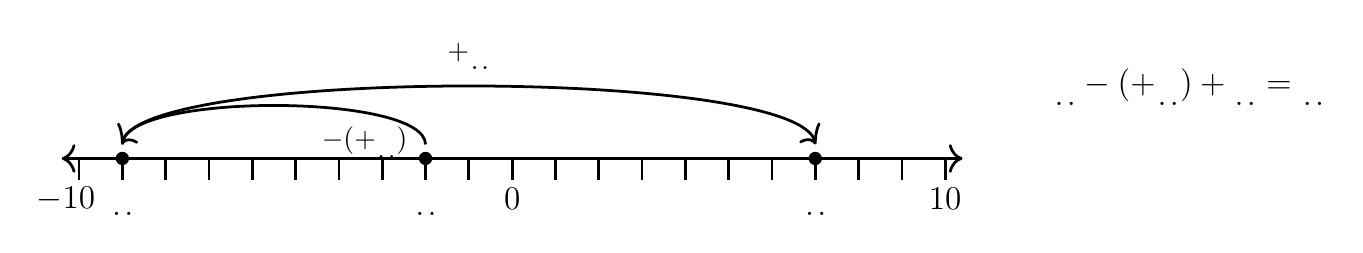
\begin{tikzpicture}[scale=0.55, baseline={([yshift=-1pt]current bounding box.north)}]
    % axis, arrow style to-to
    \draw[{To[scale=1.3]}-{To[scale=1.3]}, line width=1pt] (-10.4, 0) -- (10.4, 0);
    % tick marks
    \foreach \x in {-10,-9,...,10}
        \draw[shift={(\x,0)},color=black, line width=1pt] (0pt,-14pt) -- (0pt,0pt);
    % numbers along each axis
    \foreach \x in {-10}
        \draw[shift={(\x -0.3,-0.8)},color=black] node[font=\large,text height=12pt] {$\x$};
    \foreach \x in {0,10}
        \draw[shift={(\x,-0.8)},color=black] node[font=\large,text height=12pt] {$\x$};
    % numbers for dots
    \draw[shift={(-2,-0.8)},color=black] node[font=\large,text height=12pt] {$\qgap$};
    \draw[shift={(-9,-0.8)},color=black] node[font=\large,text height=12pt] {$\qgap$};
    \draw[shift={(7,-0.8)},color=black] node[font=\large,text height=12pt] {$\qgap$};
    % dots
    \filldraw[black] (-2,0) circle (4pt) node[above,yshift=-2pt] (a) {};
    \filldraw[black] (-9,0) circle (4pt) node[above,yshift=-2pt] (m) {};
    \filldraw[black] (7,0) circle (4pt) node[above,yshift=-2pt] (b) {};

    % first arrow (label below to left)
    \draw[-{To[scale=1.3, bend]}, line width=1pt, color=black] (a.north)
        .. controls +(north:\jumpheight mm) and +(north:\jumpheight mm) ..
        node[above=-9pt, xshift=-22pt, font=\normalsize, text height=8pt, pos=0] {$-(+\qgap)$} (m.north);

    % second arrow (label above)
    \draw[-{To[scale=1.3, bend]}, line width=1pt, color=black] (m.north)
        .. controls +(north:\jumpheighthigh mm) and +(north:\jumpheighthigh mm) ..
        node[above=2pt, font=\normalsize, text height=8pt] {$+\qgap$} (b.north);

    % equation at right end
    \node [font=\large, anchor=east] at (19,1.65) {$\qgap-(+\qgap)+\qgap = \qgap$};
\end{tikzpicture}
\end{equation}
\vspace{-2pt}\begin{equation}
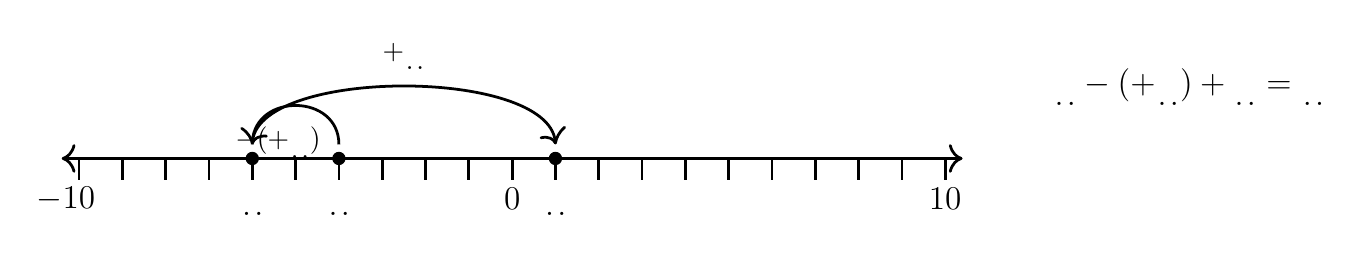
\begin{tikzpicture}[scale=0.55, baseline={([yshift=-1pt]current bounding box.north)}]
    % axis, arrow style to-to
    \draw[{To[scale=1.3]}-{To[scale=1.3]}, line width=1pt] (-10.4, 0) -- (10.4, 0);
    % tick marks
    \foreach \x in {-10,-9,...,10}
        \draw[shift={(\x,0)},color=black, line width=1pt] (0pt,-14pt) -- (0pt,0pt);
    % numbers along each axis
    \foreach \x in {-10}
        \draw[shift={(\x -0.3,-0.8)},color=black] node[font=\large,text height=12pt] {$\x$};
    \foreach \x in {0,10}
        \draw[shift={(\x,-0.8)},color=black] node[font=\large,text height=12pt] {$\x$};
    % numbers for dots
    \draw[shift={(-4,-0.8)},color=black] node[font=\large,text height=12pt] {$\qgap$};
    \draw[shift={(-6,-0.8)},color=black] node[font=\large,text height=12pt] {$\qgap$};
    \draw[shift={(1,-0.8)},color=black] node[font=\large,text height=12pt] {$\qgap$};
    % dots
    \filldraw[black] (-4,0) circle (4pt) node[above,yshift=-2pt] (a) {};
    \filldraw[black] (-6,0) circle (4pt) node[above,yshift=-2pt] (m) {};
    \filldraw[black] (1,0) circle (4pt) node[above,yshift=-2pt] (b) {};

    % first arrow (label below to left)
    \draw[-{To[scale=1.3, bend]}, line width=1pt, color=black] (a.north)
        .. controls +(north:\jumpheight mm) and +(north:\jumpheight mm) ..
        node[above=-9pt, xshift=-22pt, font=\normalsize, text height=8pt, pos=0] {$-(+\qgap)$} (m.north);

    % second arrow (label above)
    \draw[-{To[scale=1.3, bend]}, line width=1pt, color=black] (m.north)
        .. controls +(north:\jumpheighthigh mm) and +(north:\jumpheighthigh mm) ..
        node[above=2pt, font=\normalsize, text height=8pt] {$+\qgap$} (b.north);

    % equation at right end
    \node [font=\large, anchor=east] at (19,1.65) {$\qgap-(+\qgap)+\qgap = \qgap$};
\end{tikzpicture}
\end{equation}
\vspace{-2pt}\begin{equation}
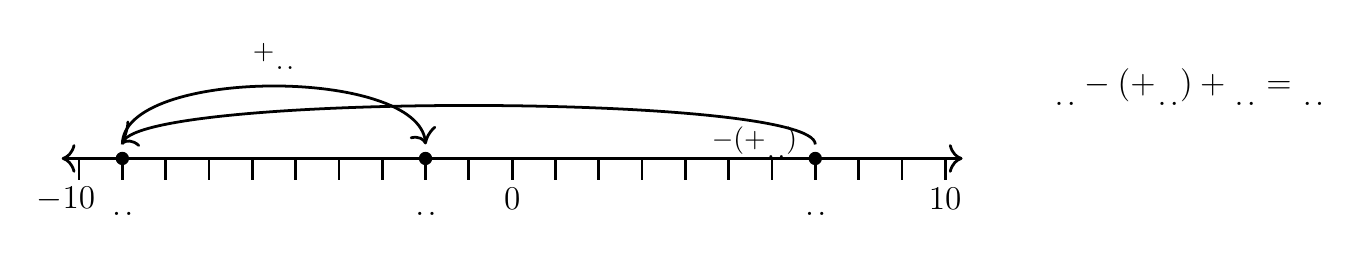
\begin{tikzpicture}[scale=0.55, baseline={([yshift=-1pt]current bounding box.north)}]
    % axis, arrow style to-to
    \draw[{To[scale=1.3]}-{To[scale=1.3]}, line width=1pt] (-10.4, 0) -- (10.4, 0);
    % tick marks
    \foreach \x in {-10,-9,...,10}
        \draw[shift={(\x,0)},color=black, line width=1pt] (0pt,-14pt) -- (0pt,0pt);
    % numbers along each axis
    \foreach \x in {-10}
        \draw[shift={(\x -0.3,-0.8)},color=black] node[font=\large,text height=12pt] {$\x$};
    \foreach \x in {0,10}
        \draw[shift={(\x,-0.8)},color=black] node[font=\large,text height=12pt] {$\x$};
    % numbers for dots
    \draw[shift={(7,-0.8)},color=black] node[font=\large,text height=12pt] {$\qgap$};
    \draw[shift={(-9,-0.8)},color=black] node[font=\large,text height=12pt] {$\qgap$};
    \draw[shift={(-2,-0.8)},color=black] node[font=\large,text height=12pt] {$\qgap$};
    % dots
    \filldraw[black] (7,0) circle (4pt) node[above,yshift=-2pt] (a) {};
    \filldraw[black] (-9,0) circle (4pt) node[above,yshift=-2pt] (m) {};
    \filldraw[black] (-2,0) circle (4pt) node[above,yshift=-2pt] (b) {};

    % first arrow (label below to left)
    \draw[-{To[scale=1.3, bend]}, line width=1pt, color=black] (a.north)
        .. controls +(north:\jumpheight mm) and +(north:\jumpheight mm) ..
        node[above=-9pt, xshift=-22pt, font=\normalsize, text height=8pt, pos=0] {$-(+\qgap)$} (m.north);

    % second arrow (label above)
    \draw[-{To[scale=1.3, bend]}, line width=1pt, color=black] (m.north)
        .. controls +(north:\jumpheighthigh mm) and +(north:\jumpheighthigh mm) ..
        node[above=2pt, font=\normalsize, text height=8pt] {$+\qgap$} (b.north);

    % equation at right end
    \node [font=\large, anchor=east] at (19,1.65) {$\qgap-(+\qgap)+\qgap = \qgap$};
\end{tikzpicture}
\end{equation}
\vspace{-2pt}\begin{equation}
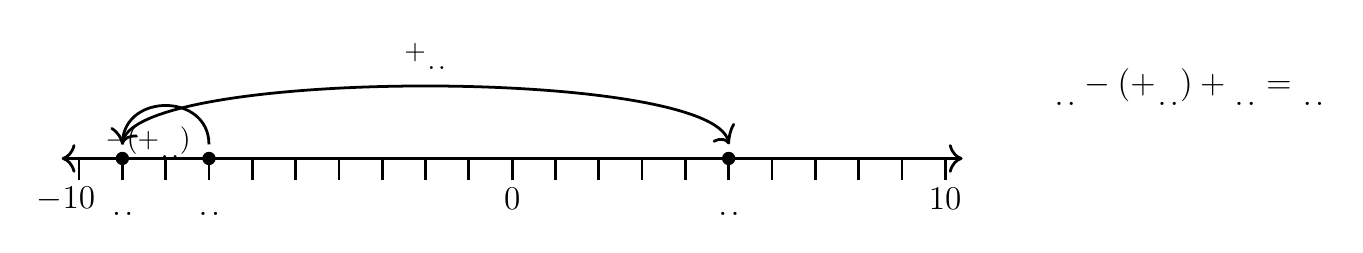
\begin{tikzpicture}[scale=0.55, baseline={([yshift=-1pt]current bounding box.north)}]
    % axis, arrow style to-to
    \draw[{To[scale=1.3]}-{To[scale=1.3]}, line width=1pt] (-10.4, 0) -- (10.4, 0);
    % tick marks
    \foreach \x in {-10,-9,...,10}
        \draw[shift={(\x,0)},color=black, line width=1pt] (0pt,-14pt) -- (0pt,0pt);
    % numbers along each axis
    \foreach \x in {-10}
        \draw[shift={(\x -0.3,-0.8)},color=black] node[font=\large,text height=12pt] {$\x$};
    \foreach \x in {0,10}
        \draw[shift={(\x,-0.8)},color=black] node[font=\large,text height=12pt] {$\x$};
    % numbers for dots
    \draw[shift={(-7,-0.8)},color=black] node[font=\large,text height=12pt] {$\qgap$};
    \draw[shift={(-9,-0.8)},color=black] node[font=\large,text height=12pt] {$\qgap$};
    \draw[shift={(5,-0.8)},color=black] node[font=\large,text height=12pt] {$\qgap$};
    % dots
    \filldraw[black] (-7,0) circle (4pt) node[above,yshift=-2pt] (a) {};
    \filldraw[black] (-9,0) circle (4pt) node[above,yshift=-2pt] (m) {};
    \filldraw[black] (5,0) circle (4pt) node[above,yshift=-2pt] (b) {};

    % first arrow (label below to left)
    \draw[-{To[scale=1.3, bend]}, line width=1pt, color=black] (a.north)
        .. controls +(north:\jumpheight mm) and +(north:\jumpheight mm) ..
        node[above=-9pt, xshift=-22pt, font=\normalsize, text height=8pt, pos=0] {$-(+\qgap)$} (m.north);

    % second arrow (label above)
    \draw[-{To[scale=1.3, bend]}, line width=1pt, color=black] (m.north)
        .. controls +(north:\jumpheighthigh mm) and +(north:\jumpheighthigh mm) ..
        node[above=2pt, font=\normalsize, text height=8pt] {$+\qgap$} (b.north);

    % equation at right end
    \node [font=\large, anchor=east] at (19,1.65) {$\qgap-(+\qgap)+\qgap = \qgap$};
\end{tikzpicture}
\end{equation}
\vspace{-2pt}\begin{equation}
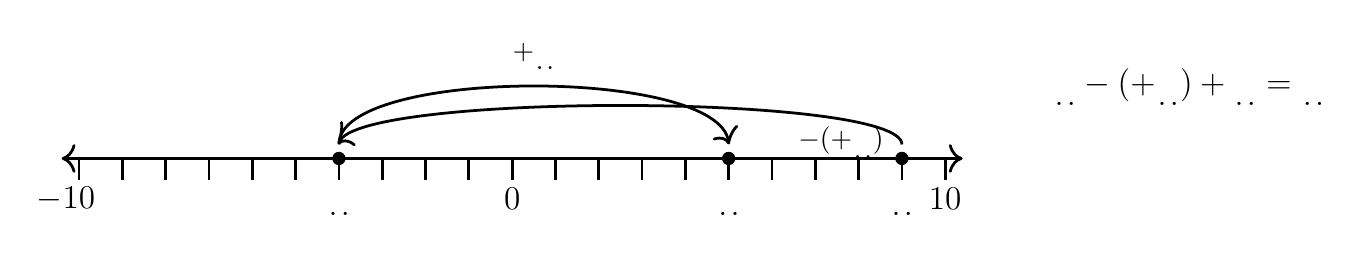
\begin{tikzpicture}[scale=0.55, baseline={([yshift=-1pt]current bounding box.north)}]
    % axis, arrow style to-to
    \draw[{To[scale=1.3]}-{To[scale=1.3]}, line width=1pt] (-10.4, 0) -- (10.4, 0);
    % tick marks
    \foreach \x in {-10,-9,...,10}
        \draw[shift={(\x,0)},color=black, line width=1pt] (0pt,-14pt) -- (0pt,0pt);
    % numbers along each axis
    \foreach \x in {-10}
        \draw[shift={(\x -0.3,-0.8)},color=black] node[font=\large,text height=12pt] {$\x$};
    \foreach \x in {0,10}
        \draw[shift={(\x,-0.8)},color=black] node[font=\large,text height=12pt] {$\x$};
    % numbers for dots
    \draw[shift={(9,-0.8)},color=black] node[font=\large,text height=12pt] {$\qgap$};
    \draw[shift={(-4,-0.8)},color=black] node[font=\large,text height=12pt] {$\qgap$};
    \draw[shift={(5,-0.8)},color=black] node[font=\large,text height=12pt] {$\qgap$};
    % dots
    \filldraw[black] (9,0) circle (4pt) node[above,yshift=-2pt] (a) {};
    \filldraw[black] (-4,0) circle (4pt) node[above,yshift=-2pt] (m) {};
    \filldraw[black] (5,0) circle (4pt) node[above,yshift=-2pt] (b) {};

    % first arrow (label below to left)
    \draw[-{To[scale=1.3, bend]}, line width=1pt, color=black] (a.north)
        .. controls +(north:\jumpheight mm) and +(north:\jumpheight mm) ..
        node[above=-9pt, xshift=-22pt, font=\normalsize, text height=8pt, pos=0] {$-(+\qgap)$} (m.north);

    % second arrow (label above)
    \draw[-{To[scale=1.3, bend]}, line width=1pt, color=black] (m.north)
        .. controls +(north:\jumpheighthigh mm) and +(north:\jumpheighthigh mm) ..
        node[above=2pt, font=\normalsize, text height=8pt] {$+\qgap$} (b.north);

    % equation at right end
    \node [font=\large, anchor=east] at (19,1.65) {$\qgap-(+\qgap)+\qgap = \qgap$};
\end{tikzpicture}
\end{equation}
\vspace{-2pt}\pagebreak ~ \newline ~ \newline\begin{equation}
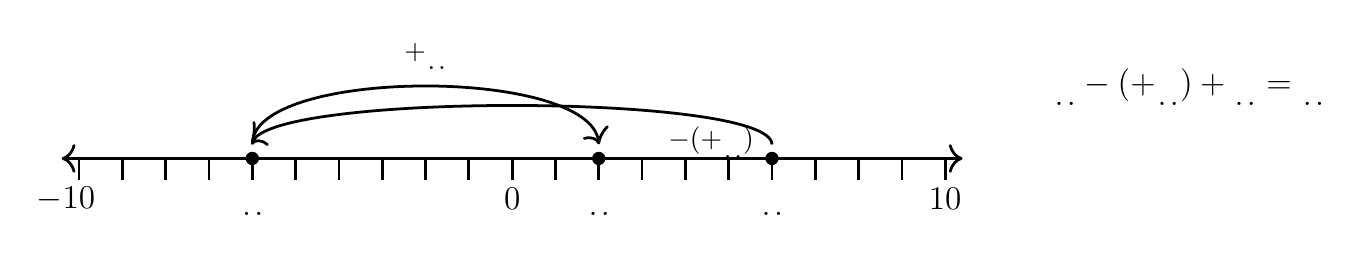
\begin{tikzpicture}[scale=0.55, baseline={([yshift=-1pt]current bounding box.north)}]
    % axis, arrow style to-to
    \draw[{To[scale=1.3]}-{To[scale=1.3]}, line width=1pt] (-10.4, 0) -- (10.4, 0);
    % tick marks
    \foreach \x in {-10,-9,...,10}
        \draw[shift={(\x,0)},color=black, line width=1pt] (0pt,-14pt) -- (0pt,0pt);
    % numbers along each axis
    \foreach \x in {-10}
        \draw[shift={(\x -0.3,-0.8)},color=black] node[font=\large,text height=12pt] {$\x$};
    \foreach \x in {0,10}
        \draw[shift={(\x,-0.8)},color=black] node[font=\large,text height=12pt] {$\x$};
    % numbers for dots
    \draw[shift={(6,-0.8)},color=black] node[font=\large,text height=12pt] {$\qgap$};
    \draw[shift={(-6,-0.8)},color=black] node[font=\large,text height=12pt] {$\qgap$};
    \draw[shift={(2,-0.8)},color=black] node[font=\large,text height=12pt] {$\qgap$};
    % dots
    \filldraw[black] (6,0) circle (4pt) node[above,yshift=-2pt] (a) {};
    \filldraw[black] (-6,0) circle (4pt) node[above,yshift=-2pt] (m) {};
    \filldraw[black] (2,0) circle (4pt) node[above,yshift=-2pt] (b) {};

    % first arrow (label below to left)
    \draw[-{To[scale=1.3, bend]}, line width=1pt, color=black] (a.north)
        .. controls +(north:\jumpheight mm) and +(north:\jumpheight mm) ..
        node[above=-9pt, xshift=-22pt, font=\normalsize, text height=8pt, pos=0] {$-(+\qgap)$} (m.north);

    % second arrow (label above)
    \draw[-{To[scale=1.3, bend]}, line width=1pt, color=black] (m.north)
        .. controls +(north:\jumpheighthigh mm) and +(north:\jumpheighthigh mm) ..
        node[above=2pt, font=\normalsize, text height=8pt] {$+\qgap$} (b.north);

    % equation at right end
    \node [font=\large, anchor=east] at (19,1.65) {$\qgap-(+\qgap)+\qgap = \qgap$};
\end{tikzpicture}
\end{equation}
\vspace{-2pt}\begin{equation}
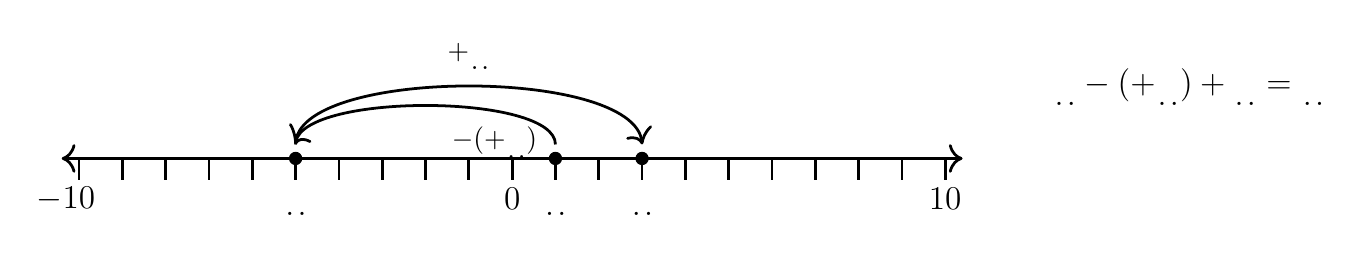
\begin{tikzpicture}[scale=0.55, baseline={([yshift=-1pt]current bounding box.north)}]
    % axis, arrow style to-to
    \draw[{To[scale=1.3]}-{To[scale=1.3]}, line width=1pt] (-10.4, 0) -- (10.4, 0);
    % tick marks
    \foreach \x in {-10,-9,...,10}
        \draw[shift={(\x,0)},color=black, line width=1pt] (0pt,-14pt) -- (0pt,0pt);
    % numbers along each axis
    \foreach \x in {-10}
        \draw[shift={(\x -0.3,-0.8)},color=black] node[font=\large,text height=12pt] {$\x$};
    \foreach \x in {0,10}
        \draw[shift={(\x,-0.8)},color=black] node[font=\large,text height=12pt] {$\x$};
    % numbers for dots
    \draw[shift={(1,-0.8)},color=black] node[font=\large,text height=12pt] {$\qgap$};
    \draw[shift={(-5,-0.8)},color=black] node[font=\large,text height=12pt] {$\qgap$};
    \draw[shift={(3,-0.8)},color=black] node[font=\large,text height=12pt] {$\qgap$};
    % dots
    \filldraw[black] (1,0) circle (4pt) node[above,yshift=-2pt] (a) {};
    \filldraw[black] (-5,0) circle (4pt) node[above,yshift=-2pt] (m) {};
    \filldraw[black] (3,0) circle (4pt) node[above,yshift=-2pt] (b) {};

    % first arrow (label below to left)
    \draw[-{To[scale=1.3, bend]}, line width=1pt, color=black] (a.north)
        .. controls +(north:\jumpheight mm) and +(north:\jumpheight mm) ..
        node[above=-9pt, xshift=-22pt, font=\normalsize, text height=8pt, pos=0] {$-(+\qgap)$} (m.north);

    % second arrow (label above)
    \draw[-{To[scale=1.3, bend]}, line width=1pt, color=black] (m.north)
        .. controls +(north:\jumpheighthigh mm) and +(north:\jumpheighthigh mm) ..
        node[above=2pt, font=\normalsize, text height=8pt] {$+\qgap$} (b.north);

    % equation at right end
    \node [font=\large, anchor=east] at (19,1.65) {$\qgap-(+\qgap)+\qgap = \qgap$};
\end{tikzpicture}
\end{equation}
\vspace{-2pt}\begin{equation}
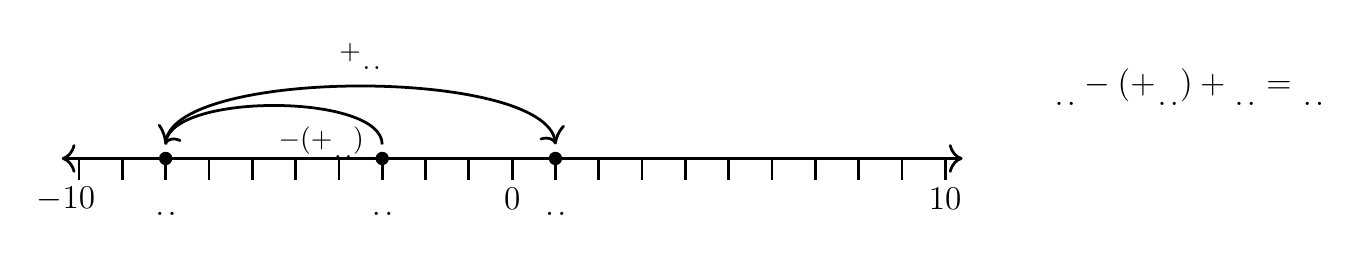
\begin{tikzpicture}[scale=0.55, baseline={([yshift=-1pt]current bounding box.north)}]
    % axis, arrow style to-to
    \draw[{To[scale=1.3]}-{To[scale=1.3]}, line width=1pt] (-10.4, 0) -- (10.4, 0);
    % tick marks
    \foreach \x in {-10,-9,...,10}
        \draw[shift={(\x,0)},color=black, line width=1pt] (0pt,-14pt) -- (0pt,0pt);
    % numbers along each axis
    \foreach \x in {-10}
        \draw[shift={(\x -0.3,-0.8)},color=black] node[font=\large,text height=12pt] {$\x$};
    \foreach \x in {0,10}
        \draw[shift={(\x,-0.8)},color=black] node[font=\large,text height=12pt] {$\x$};
    % numbers for dots
    \draw[shift={(-3,-0.8)},color=black] node[font=\large,text height=12pt] {$\qgap$};
    \draw[shift={(-8,-0.8)},color=black] node[font=\large,text height=12pt] {$\qgap$};
    \draw[shift={(1,-0.8)},color=black] node[font=\large,text height=12pt] {$\qgap$};
    % dots
    \filldraw[black] (-3,0) circle (4pt) node[above,yshift=-2pt] (a) {};
    \filldraw[black] (-8,0) circle (4pt) node[above,yshift=-2pt] (m) {};
    \filldraw[black] (1,0) circle (4pt) node[above,yshift=-2pt] (b) {};

    % first arrow (label below to left)
    \draw[-{To[scale=1.3, bend]}, line width=1pt, color=black] (a.north)
        .. controls +(north:\jumpheight mm) and +(north:\jumpheight mm) ..
        node[above=-9pt, xshift=-22pt, font=\normalsize, text height=8pt, pos=0] {$-(+\qgap)$} (m.north);

    % second arrow (label above)
    \draw[-{To[scale=1.3, bend]}, line width=1pt, color=black] (m.north)
        .. controls +(north:\jumpheighthigh mm) and +(north:\jumpheighthigh mm) ..
        node[above=2pt, font=\normalsize, text height=8pt] {$+\qgap$} (b.north);

    % equation at right end
    \node [font=\large, anchor=east] at (19,1.65) {$\qgap-(+\qgap)+\qgap = \qgap$};
\end{tikzpicture}
\end{equation}
\vspace{-2pt}\begin{equation}
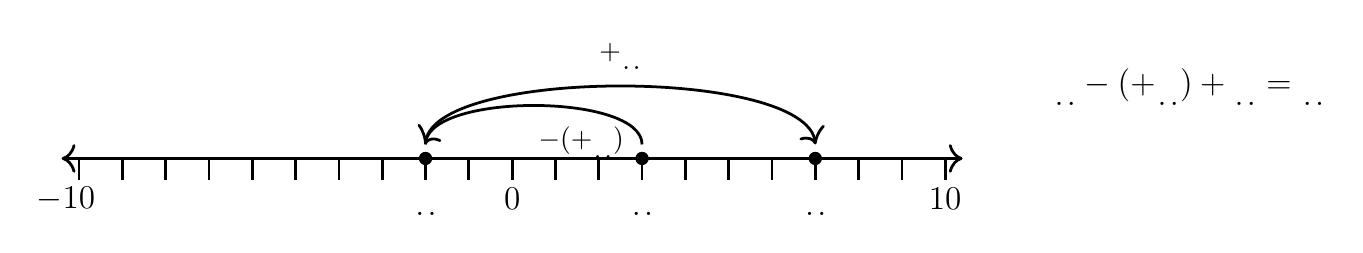
\begin{tikzpicture}[scale=0.55, baseline={([yshift=-1pt]current bounding box.north)}]
    % axis, arrow style to-to
    \draw[{To[scale=1.3]}-{To[scale=1.3]}, line width=1pt] (-10.4, 0) -- (10.4, 0);
    % tick marks
    \foreach \x in {-10,-9,...,10}
        \draw[shift={(\x,0)},color=black, line width=1pt] (0pt,-14pt) -- (0pt,0pt);
    % numbers along each axis
    \foreach \x in {-10}
        \draw[shift={(\x -0.3,-0.8)},color=black] node[font=\large,text height=12pt] {$\x$};
    \foreach \x in {0,10}
        \draw[shift={(\x,-0.8)},color=black] node[font=\large,text height=12pt] {$\x$};
    % numbers for dots
    \draw[shift={(3,-0.8)},color=black] node[font=\large,text height=12pt] {$\qgap$};
    \draw[shift={(-2,-0.8)},color=black] node[font=\large,text height=12pt] {$\qgap$};
    \draw[shift={(7,-0.8)},color=black] node[font=\large,text height=12pt] {$\qgap$};
    % dots
    \filldraw[black] (3,0) circle (4pt) node[above,yshift=-2pt] (a) {};
    \filldraw[black] (-2,0) circle (4pt) node[above,yshift=-2pt] (m) {};
    \filldraw[black] (7,0) circle (4pt) node[above,yshift=-2pt] (b) {};

    % first arrow (label below to left)
    \draw[-{To[scale=1.3, bend]}, line width=1pt, color=black] (a.north)
        .. controls +(north:\jumpheight mm) and +(north:\jumpheight mm) ..
        node[above=-9pt, xshift=-22pt, font=\normalsize, text height=8pt, pos=0] {$-(+\qgap)$} (m.north);

    % second arrow (label above)
    \draw[-{To[scale=1.3, bend]}, line width=1pt, color=black] (m.north)
        .. controls +(north:\jumpheighthigh mm) and +(north:\jumpheighthigh mm) ..
        node[above=2pt, font=\normalsize, text height=8pt] {$+\qgap$} (b.north);

    % equation at right end
    \node [font=\large, anchor=east] at (19,1.65) {$\qgap-(+\qgap)+\qgap = \qgap$};
\end{tikzpicture}
\end{equation}
\vspace{-2pt}\begin{equation}
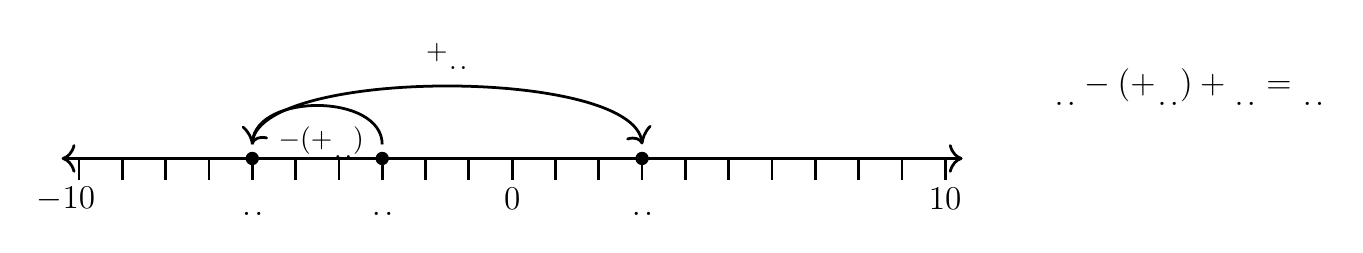
\begin{tikzpicture}[scale=0.55, baseline={([yshift=-1pt]current bounding box.north)}]
    % axis, arrow style to-to
    \draw[{To[scale=1.3]}-{To[scale=1.3]}, line width=1pt] (-10.4, 0) -- (10.4, 0);
    % tick marks
    \foreach \x in {-10,-9,...,10}
        \draw[shift={(\x,0)},color=black, line width=1pt] (0pt,-14pt) -- (0pt,0pt);
    % numbers along each axis
    \foreach \x in {-10}
        \draw[shift={(\x -0.3,-0.8)},color=black] node[font=\large,text height=12pt] {$\x$};
    \foreach \x in {0,10}
        \draw[shift={(\x,-0.8)},color=black] node[font=\large,text height=12pt] {$\x$};
    % numbers for dots
    \draw[shift={(-3,-0.8)},color=black] node[font=\large,text height=12pt] {$\qgap$};
    \draw[shift={(-6,-0.8)},color=black] node[font=\large,text height=12pt] {$\qgap$};
    \draw[shift={(3,-0.8)},color=black] node[font=\large,text height=12pt] {$\qgap$};
    % dots
    \filldraw[black] (-3,0) circle (4pt) node[above,yshift=-2pt] (a) {};
    \filldraw[black] (-6,0) circle (4pt) node[above,yshift=-2pt] (m) {};
    \filldraw[black] (3,0) circle (4pt) node[above,yshift=-2pt] (b) {};

    % first arrow (label below to left)
    \draw[-{To[scale=1.3, bend]}, line width=1pt, color=black] (a.north)
        .. controls +(north:\jumpheight mm) and +(north:\jumpheight mm) ..
        node[above=-9pt, xshift=-22pt, font=\normalsize, text height=8pt, pos=0] {$-(+\qgap)$} (m.north);

    % second arrow (label above)
    \draw[-{To[scale=1.3, bend]}, line width=1pt, color=black] (m.north)
        .. controls +(north:\jumpheighthigh mm) and +(north:\jumpheighthigh mm) ..
        node[above=2pt, font=\normalsize, text height=8pt] {$+\qgap$} (b.north);

    % equation at right end
    \node [font=\large, anchor=east] at (19,1.65) {$\qgap-(+\qgap)+\qgap = \qgap$};
\end{tikzpicture}
\end{equation}
\vspace{-2pt}\begin{equation}
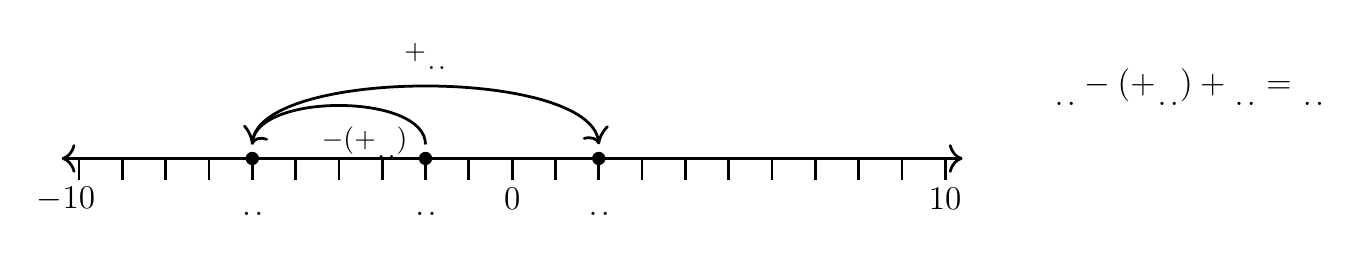
\begin{tikzpicture}[scale=0.55, baseline={([yshift=-1pt]current bounding box.north)}]
    % axis, arrow style to-to
    \draw[{To[scale=1.3]}-{To[scale=1.3]}, line width=1pt] (-10.4, 0) -- (10.4, 0);
    % tick marks
    \foreach \x in {-10,-9,...,10}
        \draw[shift={(\x,0)},color=black, line width=1pt] (0pt,-14pt) -- (0pt,0pt);
    % numbers along each axis
    \foreach \x in {-10}
        \draw[shift={(\x -0.3,-0.8)},color=black] node[font=\large,text height=12pt] {$\x$};
    \foreach \x in {0,10}
        \draw[shift={(\x,-0.8)},color=black] node[font=\large,text height=12pt] {$\x$};
    % numbers for dots
    \draw[shift={(-2,-0.8)},color=black] node[font=\large,text height=12pt] {$\qgap$};
    \draw[shift={(-6,-0.8)},color=black] node[font=\large,text height=12pt] {$\qgap$};
    \draw[shift={(2,-0.8)},color=black] node[font=\large,text height=12pt] {$\qgap$};
    % dots
    \filldraw[black] (-2,0) circle (4pt) node[above,yshift=-2pt] (a) {};
    \filldraw[black] (-6,0) circle (4pt) node[above,yshift=-2pt] (m) {};
    \filldraw[black] (2,0) circle (4pt) node[above,yshift=-2pt] (b) {};

    % first arrow (label below to left)
    \draw[-{To[scale=1.3, bend]}, line width=1pt, color=black] (a.north)
        .. controls +(north:\jumpheight mm) and +(north:\jumpheight mm) ..
        node[above=-9pt, xshift=-22pt, font=\normalsize, text height=8pt, pos=0] {$-(+\qgap)$} (m.north);

    % second arrow (label above)
    \draw[-{To[scale=1.3, bend]}, line width=1pt, color=black] (m.north)
        .. controls +(north:\jumpheighthigh mm) and +(north:\jumpheighthigh mm) ..
        node[above=2pt, font=\normalsize, text height=8pt] {$+\qgap$} (b.north);

    % equation at right end
    \node [font=\large, anchor=east] at (19,1.65) {$\qgap-(+\qgap)+\qgap = \qgap$};
\end{tikzpicture}
\end{equation}
\vspace{-2pt}\begin{equation}
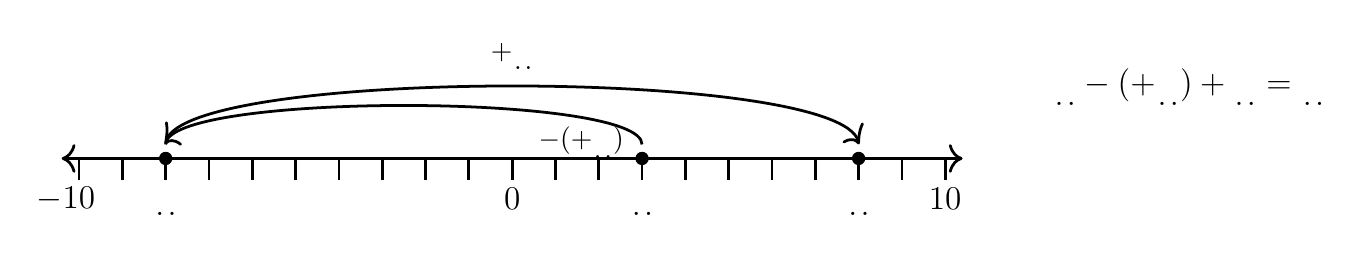
\begin{tikzpicture}[scale=0.55, baseline={([yshift=-1pt]current bounding box.north)}]
    % axis, arrow style to-to
    \draw[{To[scale=1.3]}-{To[scale=1.3]}, line width=1pt] (-10.4, 0) -- (10.4, 0);
    % tick marks
    \foreach \x in {-10,-9,...,10}
        \draw[shift={(\x,0)},color=black, line width=1pt] (0pt,-14pt) -- (0pt,0pt);
    % numbers along each axis
    \foreach \x in {-10}
        \draw[shift={(\x -0.3,-0.8)},color=black] node[font=\large,text height=12pt] {$\x$};
    \foreach \x in {0,10}
        \draw[shift={(\x,-0.8)},color=black] node[font=\large,text height=12pt] {$\x$};
    % numbers for dots
    \draw[shift={(3,-0.8)},color=black] node[font=\large,text height=12pt] {$\qgap$};
    \draw[shift={(-8,-0.8)},color=black] node[font=\large,text height=12pt] {$\qgap$};
    \draw[shift={(8,-0.8)},color=black] node[font=\large,text height=12pt] {$\qgap$};
    % dots
    \filldraw[black] (3,0) circle (4pt) node[above,yshift=-2pt] (a) {};
    \filldraw[black] (-8,0) circle (4pt) node[above,yshift=-2pt] (m) {};
    \filldraw[black] (8,0) circle (4pt) node[above,yshift=-2pt] (b) {};

    % first arrow (label below to left)
    \draw[-{To[scale=1.3, bend]}, line width=1pt, color=black] (a.north)
        .. controls +(north:\jumpheight mm) and +(north:\jumpheight mm) ..
        node[above=-9pt, xshift=-22pt, font=\normalsize, text height=8pt, pos=0] {$-(+\qgap)$} (m.north);

    % second arrow (label above)
    \draw[-{To[scale=1.3, bend]}, line width=1pt, color=black] (m.north)
        .. controls +(north:\jumpheighthigh mm) and +(north:\jumpheighthigh mm) ..
        node[above=2pt, font=\normalsize, text height=8pt] {$+\qgap$} (b.north);

    % equation at right end
    \node [font=\large, anchor=east] at (19,1.65) {$\qgap-(+\qgap)+\qgap = \qgap$};
\end{tikzpicture}
\end{equation}
\vspace{-2pt}\begin{equation}
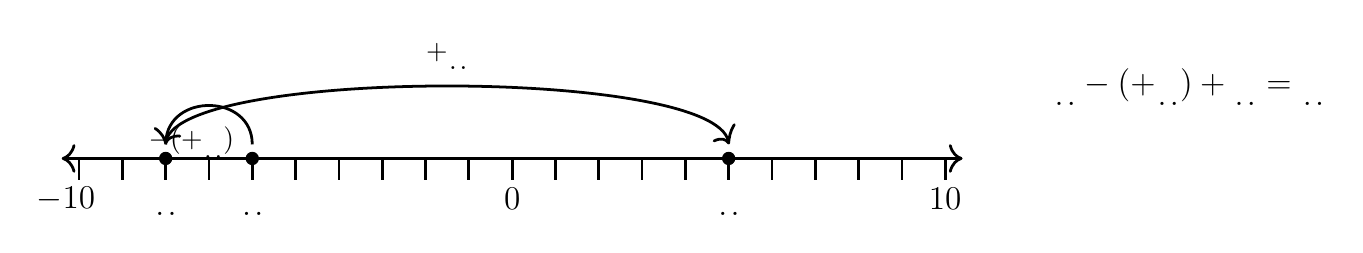
\begin{tikzpicture}[scale=0.55, baseline={([yshift=-1pt]current bounding box.north)}]
    % axis, arrow style to-to
    \draw[{To[scale=1.3]}-{To[scale=1.3]}, line width=1pt] (-10.4, 0) -- (10.4, 0);
    % tick marks
    \foreach \x in {-10,-9,...,10}
        \draw[shift={(\x,0)},color=black, line width=1pt] (0pt,-14pt) -- (0pt,0pt);
    % numbers along each axis
    \foreach \x in {-10}
        \draw[shift={(\x -0.3,-0.8)},color=black] node[font=\large,text height=12pt] {$\x$};
    \foreach \x in {0,10}
        \draw[shift={(\x,-0.8)},color=black] node[font=\large,text height=12pt] {$\x$};
    % numbers for dots
    \draw[shift={(-6,-0.8)},color=black] node[font=\large,text height=12pt] {$\qgap$};
    \draw[shift={(-8,-0.8)},color=black] node[font=\large,text height=12pt] {$\qgap$};
    \draw[shift={(5,-0.8)},color=black] node[font=\large,text height=12pt] {$\qgap$};
    % dots
    \filldraw[black] (-6,0) circle (4pt) node[above,yshift=-2pt] (a) {};
    \filldraw[black] (-8,0) circle (4pt) node[above,yshift=-2pt] (m) {};
    \filldraw[black] (5,0) circle (4pt) node[above,yshift=-2pt] (b) {};

    % first arrow (label below to left)
    \draw[-{To[scale=1.3, bend]}, line width=1pt, color=black] (a.north)
        .. controls +(north:\jumpheight mm) and +(north:\jumpheight mm) ..
        node[above=-9pt, xshift=-22pt, font=\normalsize, text height=8pt, pos=0] {$-(+\qgap)$} (m.north);

    % second arrow (label above)
    \draw[-{To[scale=1.3, bend]}, line width=1pt, color=black] (m.north)
        .. controls +(north:\jumpheighthigh mm) and +(north:\jumpheighthigh mm) ..
        node[above=2pt, font=\normalsize, text height=8pt] {$+\qgap$} (b.north);

    % equation at right end
    \node [font=\large, anchor=east] at (19,1.65) {$\qgap-(+\qgap)+\qgap = \qgap$};
\end{tikzpicture}
\end{equation}
\vspace{-2pt}\pagebreak ~ \newline ~ \newline\begin{equation}
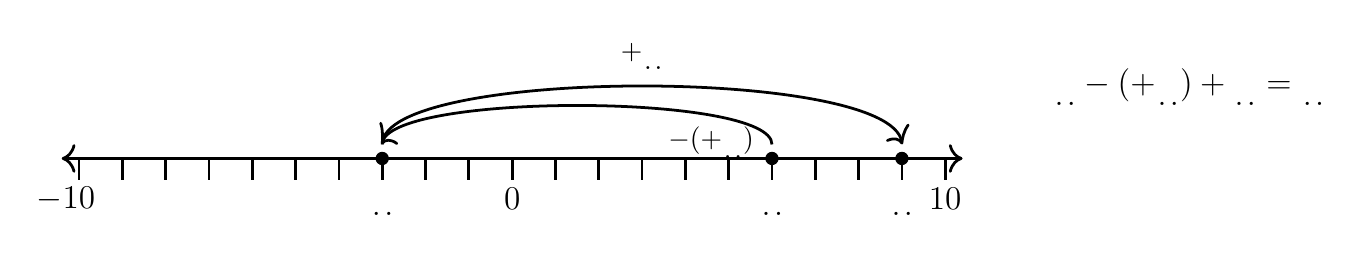
\begin{tikzpicture}[scale=0.55, baseline={([yshift=-1pt]current bounding box.north)}]
    % axis, arrow style to-to
    \draw[{To[scale=1.3]}-{To[scale=1.3]}, line width=1pt] (-10.4, 0) -- (10.4, 0);
    % tick marks
    \foreach \x in {-10,-9,...,10}
        \draw[shift={(\x,0)},color=black, line width=1pt] (0pt,-14pt) -- (0pt,0pt);
    % numbers along each axis
    \foreach \x in {-10}
        \draw[shift={(\x -0.3,-0.8)},color=black] node[font=\large,text height=12pt] {$\x$};
    \foreach \x in {0,10}
        \draw[shift={(\x,-0.8)},color=black] node[font=\large,text height=12pt] {$\x$};
    % numbers for dots
    \draw[shift={(6,-0.8)},color=black] node[font=\large,text height=12pt] {$\qgap$};
    \draw[shift={(-3,-0.8)},color=black] node[font=\large,text height=12pt] {$\qgap$};
    \draw[shift={(9,-0.8)},color=black] node[font=\large,text height=12pt] {$\qgap$};
    % dots
    \filldraw[black] (6,0) circle (4pt) node[above,yshift=-2pt] (a) {};
    \filldraw[black] (-3,0) circle (4pt) node[above,yshift=-2pt] (m) {};
    \filldraw[black] (9,0) circle (4pt) node[above,yshift=-2pt] (b) {};

    % first arrow (label below to left)
    \draw[-{To[scale=1.3, bend]}, line width=1pt, color=black] (a.north)
        .. controls +(north:\jumpheight mm) and +(north:\jumpheight mm) ..
        node[above=-9pt, xshift=-22pt, font=\normalsize, text height=8pt, pos=0] {$-(+\qgap)$} (m.north);

    % second arrow (label above)
    \draw[-{To[scale=1.3, bend]}, line width=1pt, color=black] (m.north)
        .. controls +(north:\jumpheighthigh mm) and +(north:\jumpheighthigh mm) ..
        node[above=2pt, font=\normalsize, text height=8pt] {$+\qgap$} (b.north);

    % equation at right end
    \node [font=\large, anchor=east] at (19,1.65) {$\qgap-(+\qgap)+\qgap = \qgap$};
\end{tikzpicture}
\end{equation}
\vspace{-2pt}\begin{equation}
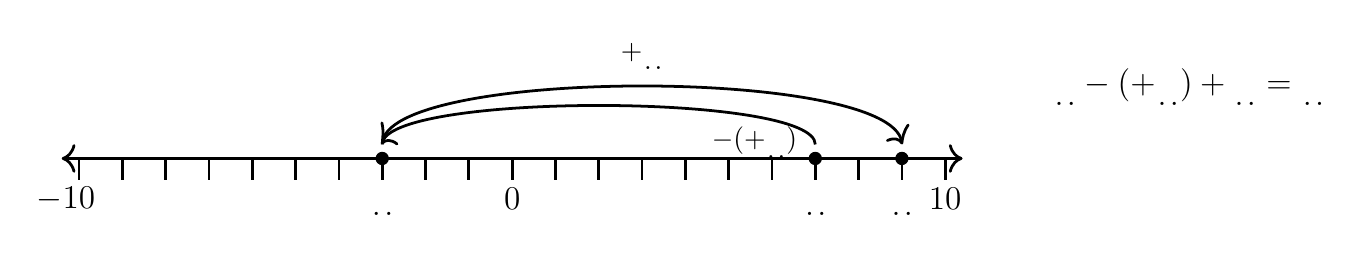
\begin{tikzpicture}[scale=0.55, baseline={([yshift=-1pt]current bounding box.north)}]
    % axis, arrow style to-to
    \draw[{To[scale=1.3]}-{To[scale=1.3]}, line width=1pt] (-10.4, 0) -- (10.4, 0);
    % tick marks
    \foreach \x in {-10,-9,...,10}
        \draw[shift={(\x,0)},color=black, line width=1pt] (0pt,-14pt) -- (0pt,0pt);
    % numbers along each axis
    \foreach \x in {-10}
        \draw[shift={(\x -0.3,-0.8)},color=black] node[font=\large,text height=12pt] {$\x$};
    \foreach \x in {0,10}
        \draw[shift={(\x,-0.8)},color=black] node[font=\large,text height=12pt] {$\x$};
    % numbers for dots
    \draw[shift={(7,-0.8)},color=black] node[font=\large,text height=12pt] {$\qgap$};
    \draw[shift={(-3,-0.8)},color=black] node[font=\large,text height=12pt] {$\qgap$};
    \draw[shift={(9,-0.8)},color=black] node[font=\large,text height=12pt] {$\qgap$};
    % dots
    \filldraw[black] (7,0) circle (4pt) node[above,yshift=-2pt] (a) {};
    \filldraw[black] (-3,0) circle (4pt) node[above,yshift=-2pt] (m) {};
    \filldraw[black] (9,0) circle (4pt) node[above,yshift=-2pt] (b) {};

    % first arrow (label below to left)
    \draw[-{To[scale=1.3, bend]}, line width=1pt, color=black] (a.north)
        .. controls +(north:\jumpheight mm) and +(north:\jumpheight mm) ..
        node[above=-9pt, xshift=-22pt, font=\normalsize, text height=8pt, pos=0] {$-(+\qgap)$} (m.north);

    % second arrow (label above)
    \draw[-{To[scale=1.3, bend]}, line width=1pt, color=black] (m.north)
        .. controls +(north:\jumpheighthigh mm) and +(north:\jumpheighthigh mm) ..
        node[above=2pt, font=\normalsize, text height=8pt] {$+\qgap$} (b.north);

    % equation at right end
    \node [font=\large, anchor=east] at (19,1.65) {$\qgap-(+\qgap)+\qgap = \qgap$};
\end{tikzpicture}
\end{equation}
\vspace{-2pt}\begin{equation}
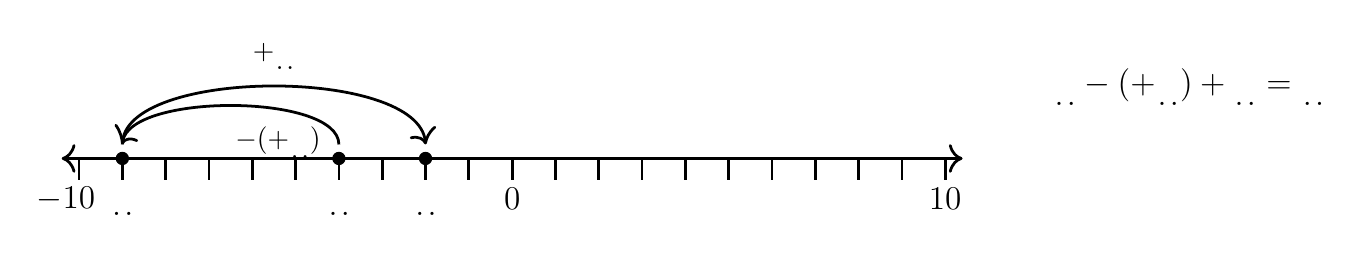
\begin{tikzpicture}[scale=0.55, baseline={([yshift=-1pt]current bounding box.north)}]
    % axis, arrow style to-to
    \draw[{To[scale=1.3]}-{To[scale=1.3]}, line width=1pt] (-10.4, 0) -- (10.4, 0);
    % tick marks
    \foreach \x in {-10,-9,...,10}
        \draw[shift={(\x,0)},color=black, line width=1pt] (0pt,-14pt) -- (0pt,0pt);
    % numbers along each axis
    \foreach \x in {-10}
        \draw[shift={(\x -0.3,-0.8)},color=black] node[font=\large,text height=12pt] {$\x$};
    \foreach \x in {0,10}
        \draw[shift={(\x,-0.8)},color=black] node[font=\large,text height=12pt] {$\x$};
    % numbers for dots
    \draw[shift={(-4,-0.8)},color=black] node[font=\large,text height=12pt] {$\qgap$};
    \draw[shift={(-9,-0.8)},color=black] node[font=\large,text height=12pt] {$\qgap$};
    \draw[shift={(-2,-0.8)},color=black] node[font=\large,text height=12pt] {$\qgap$};
    % dots
    \filldraw[black] (-4,0) circle (4pt) node[above,yshift=-2pt] (a) {};
    \filldraw[black] (-9,0) circle (4pt) node[above,yshift=-2pt] (m) {};
    \filldraw[black] (-2,0) circle (4pt) node[above,yshift=-2pt] (b) {};

    % first arrow (label below to left)
    \draw[-{To[scale=1.3, bend]}, line width=1pt, color=black] (a.north)
        .. controls +(north:\jumpheight mm) and +(north:\jumpheight mm) ..
        node[above=-9pt, xshift=-22pt, font=\normalsize, text height=8pt, pos=0] {$-(+\qgap)$} (m.north);

    % second arrow (label above)
    \draw[-{To[scale=1.3, bend]}, line width=1pt, color=black] (m.north)
        .. controls +(north:\jumpheighthigh mm) and +(north:\jumpheighthigh mm) ..
        node[above=2pt, font=\normalsize, text height=8pt] {$+\qgap$} (b.north);

    % equation at right end
    \node [font=\large, anchor=east] at (19,1.65) {$\qgap-(+\qgap)+\qgap = \qgap$};
\end{tikzpicture}
\end{equation}
\vspace{-2pt}\begin{equation}
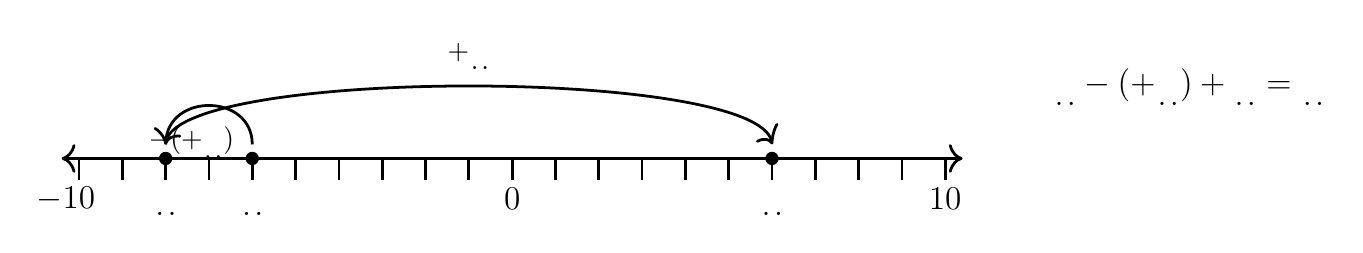
\begin{tikzpicture}[scale=0.55, baseline={([yshift=-1pt]current bounding box.north)}]
    % axis, arrow style to-to
    \draw[{To[scale=1.3]}-{To[scale=1.3]}, line width=1pt] (-10.4, 0) -- (10.4, 0);
    % tick marks
    \foreach \x in {-10,-9,...,10}
        \draw[shift={(\x,0)},color=black, line width=1pt] (0pt,-14pt) -- (0pt,0pt);
    % numbers along each axis
    \foreach \x in {-10}
        \draw[shift={(\x -0.3,-0.8)},color=black] node[font=\large,text height=12pt] {$\x$};
    \foreach \x in {0,10}
        \draw[shift={(\x,-0.8)},color=black] node[font=\large,text height=12pt] {$\x$};
    % numbers for dots
    \draw[shift={(-6,-0.8)},color=black] node[font=\large,text height=12pt] {$\qgap$};
    \draw[shift={(-8,-0.8)},color=black] node[font=\large,text height=12pt] {$\qgap$};
    \draw[shift={(6,-0.8)},color=black] node[font=\large,text height=12pt] {$\qgap$};
    % dots
    \filldraw[black] (-6,0) circle (4pt) node[above,yshift=-2pt] (a) {};
    \filldraw[black] (-8,0) circle (4pt) node[above,yshift=-2pt] (m) {};
    \filldraw[black] (6,0) circle (4pt) node[above,yshift=-2pt] (b) {};

    % first arrow (label below to left)
    \draw[-{To[scale=1.3, bend]}, line width=1pt, color=black] (a.north)
        .. controls +(north:\jumpheight mm) and +(north:\jumpheight mm) ..
        node[above=-9pt, xshift=-22pt, font=\normalsize, text height=8pt, pos=0] {$-(+\qgap)$} (m.north);

    % second arrow (label above)
    \draw[-{To[scale=1.3, bend]}, line width=1pt, color=black] (m.north)
        .. controls +(north:\jumpheighthigh mm) and +(north:\jumpheighthigh mm) ..
        node[above=2pt, font=\normalsize, text height=8pt] {$+\qgap$} (b.north);

    % equation at right end
    \node [font=\large, anchor=east] at (19,1.65) {$\qgap-(+\qgap)+\qgap = \qgap$};
\end{tikzpicture}
\end{equation}
\vspace{-2pt}\begin{equation}
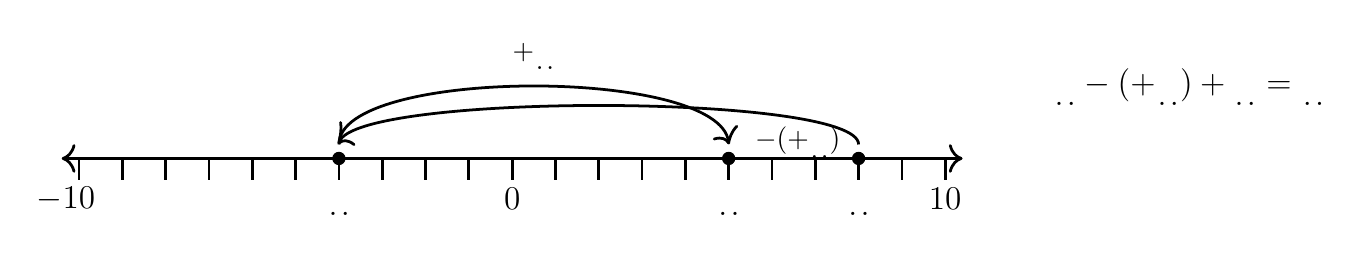
\begin{tikzpicture}[scale=0.55, baseline={([yshift=-1pt]current bounding box.north)}]
    % axis, arrow style to-to
    \draw[{To[scale=1.3]}-{To[scale=1.3]}, line width=1pt] (-10.4, 0) -- (10.4, 0);
    % tick marks
    \foreach \x in {-10,-9,...,10}
        \draw[shift={(\x,0)},color=black, line width=1pt] (0pt,-14pt) -- (0pt,0pt);
    % numbers along each axis
    \foreach \x in {-10}
        \draw[shift={(\x -0.3,-0.8)},color=black] node[font=\large,text height=12pt] {$\x$};
    \foreach \x in {0,10}
        \draw[shift={(\x,-0.8)},color=black] node[font=\large,text height=12pt] {$\x$};
    % numbers for dots
    \draw[shift={(8,-0.8)},color=black] node[font=\large,text height=12pt] {$\qgap$};
    \draw[shift={(-4,-0.8)},color=black] node[font=\large,text height=12pt] {$\qgap$};
    \draw[shift={(5,-0.8)},color=black] node[font=\large,text height=12pt] {$\qgap$};
    % dots
    \filldraw[black] (8,0) circle (4pt) node[above,yshift=-2pt] (a) {};
    \filldraw[black] (-4,0) circle (4pt) node[above,yshift=-2pt] (m) {};
    \filldraw[black] (5,0) circle (4pt) node[above,yshift=-2pt] (b) {};

    % first arrow (label below to left)
    \draw[-{To[scale=1.3, bend]}, line width=1pt, color=black] (a.north)
        .. controls +(north:\jumpheight mm) and +(north:\jumpheight mm) ..
        node[above=-9pt, xshift=-22pt, font=\normalsize, text height=8pt, pos=0] {$-(+\qgap)$} (m.north);

    % second arrow (label above)
    \draw[-{To[scale=1.3, bend]}, line width=1pt, color=black] (m.north)
        .. controls +(north:\jumpheighthigh mm) and +(north:\jumpheighthigh mm) ..
        node[above=2pt, font=\normalsize, text height=8pt] {$+\qgap$} (b.north);

    % equation at right end
    \node [font=\large, anchor=east] at (19,1.65) {$\qgap-(+\qgap)+\qgap = \qgap$};
\end{tikzpicture}
\end{equation}
\vspace{-2pt}\begin{equation}
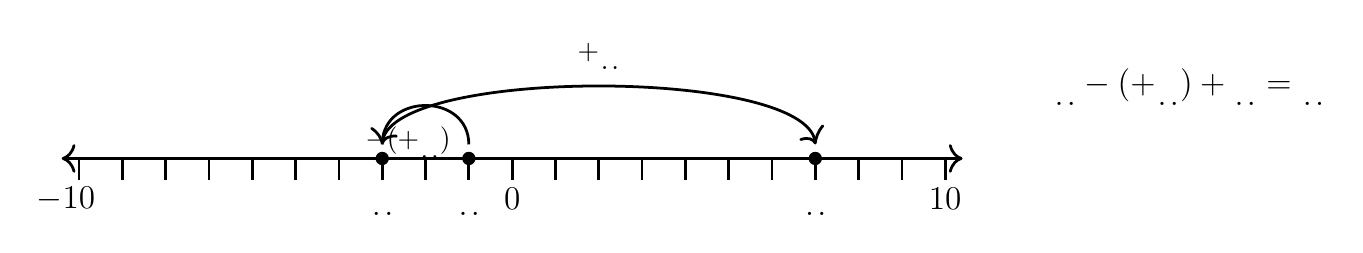
\begin{tikzpicture}[scale=0.55, baseline={([yshift=-1pt]current bounding box.north)}]
    % axis, arrow style to-to
    \draw[{To[scale=1.3]}-{To[scale=1.3]}, line width=1pt] (-10.4, 0) -- (10.4, 0);
    % tick marks
    \foreach \x in {-10,-9,...,10}
        \draw[shift={(\x,0)},color=black, line width=1pt] (0pt,-14pt) -- (0pt,0pt);
    % numbers along each axis
    \foreach \x in {-10}
        \draw[shift={(\x -0.3,-0.8)},color=black] node[font=\large,text height=12pt] {$\x$};
    \foreach \x in {0,10}
        \draw[shift={(\x,-0.8)},color=black] node[font=\large,text height=12pt] {$\x$};
    % numbers for dots
    \draw[shift={(-1,-0.8)},color=black] node[font=\large,text height=12pt] {$\qgap$};
    \draw[shift={(-3,-0.8)},color=black] node[font=\large,text height=12pt] {$\qgap$};
    \draw[shift={(7,-0.8)},color=black] node[font=\large,text height=12pt] {$\qgap$};
    % dots
    \filldraw[black] (-1,0) circle (4pt) node[above,yshift=-2pt] (a) {};
    \filldraw[black] (-3,0) circle (4pt) node[above,yshift=-2pt] (m) {};
    \filldraw[black] (7,0) circle (4pt) node[above,yshift=-2pt] (b) {};

    % first arrow (label below to left)
    \draw[-{To[scale=1.3, bend]}, line width=1pt, color=black] (a.north)
        .. controls +(north:\jumpheight mm) and +(north:\jumpheight mm) ..
        node[above=-9pt, xshift=-22pt, font=\normalsize, text height=8pt, pos=0] {$-(+\qgap)$} (m.north);

    % second arrow (label above)
    \draw[-{To[scale=1.3, bend]}, line width=1pt, color=black] (m.north)
        .. controls +(north:\jumpheighthigh mm) and +(north:\jumpheighthigh mm) ..
        node[above=2pt, font=\normalsize, text height=8pt] {$+\qgap$} (b.north);

    % equation at right end
    \node [font=\large, anchor=east] at (19,1.65) {$\qgap-(+\qgap)+\qgap = \qgap$};
\end{tikzpicture}
\end{equation}
\vspace{-2pt}\begin{equation}
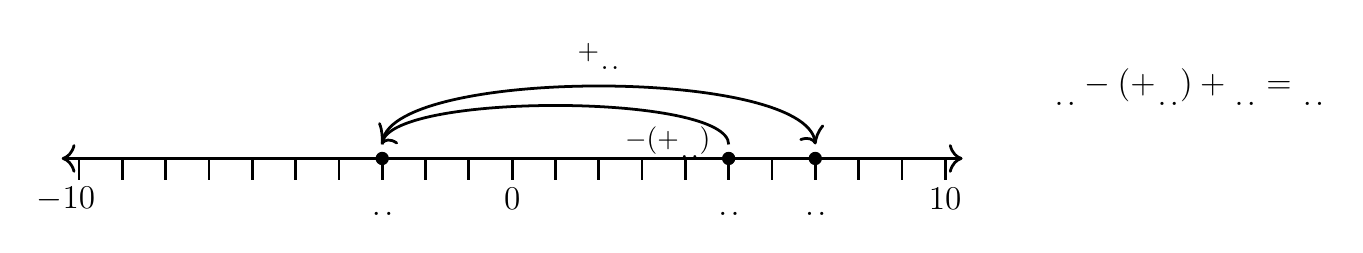
\begin{tikzpicture}[scale=0.55, baseline={([yshift=-1pt]current bounding box.north)}]
    % axis, arrow style to-to
    \draw[{To[scale=1.3]}-{To[scale=1.3]}, line width=1pt] (-10.4, 0) -- (10.4, 0);
    % tick marks
    \foreach \x in {-10,-9,...,10}
        \draw[shift={(\x,0)},color=black, line width=1pt] (0pt,-14pt) -- (0pt,0pt);
    % numbers along each axis
    \foreach \x in {-10}
        \draw[shift={(\x -0.3,-0.8)},color=black] node[font=\large,text height=12pt] {$\x$};
    \foreach \x in {0,10}
        \draw[shift={(\x,-0.8)},color=black] node[font=\large,text height=12pt] {$\x$};
    % numbers for dots
    \draw[shift={(5,-0.8)},color=black] node[font=\large,text height=12pt] {$\qgap$};
    \draw[shift={(-3,-0.8)},color=black] node[font=\large,text height=12pt] {$\qgap$};
    \draw[shift={(7,-0.8)},color=black] node[font=\large,text height=12pt] {$\qgap$};
    % dots
    \filldraw[black] (5,0) circle (4pt) node[above,yshift=-2pt] (a) {};
    \filldraw[black] (-3,0) circle (4pt) node[above,yshift=-2pt] (m) {};
    \filldraw[black] (7,0) circle (4pt) node[above,yshift=-2pt] (b) {};

    % first arrow (label below to left)
    \draw[-{To[scale=1.3, bend]}, line width=1pt, color=black] (a.north)
        .. controls +(north:\jumpheight mm) and +(north:\jumpheight mm) ..
        node[above=-9pt, xshift=-22pt, font=\normalsize, text height=8pt, pos=0] {$-(+\qgap)$} (m.north);

    % second arrow (label above)
    \draw[-{To[scale=1.3, bend]}, line width=1pt, color=black] (m.north)
        .. controls +(north:\jumpheighthigh mm) and +(north:\jumpheighthigh mm) ..
        node[above=2pt, font=\normalsize, text height=8pt] {$+\qgap$} (b.north);

    % equation at right end
    \node [font=\large, anchor=east] at (19,1.65) {$\qgap-(+\qgap)+\qgap = \qgap$};
\end{tikzpicture}
\end{equation}
\vspace{-2pt}\begin{equation}
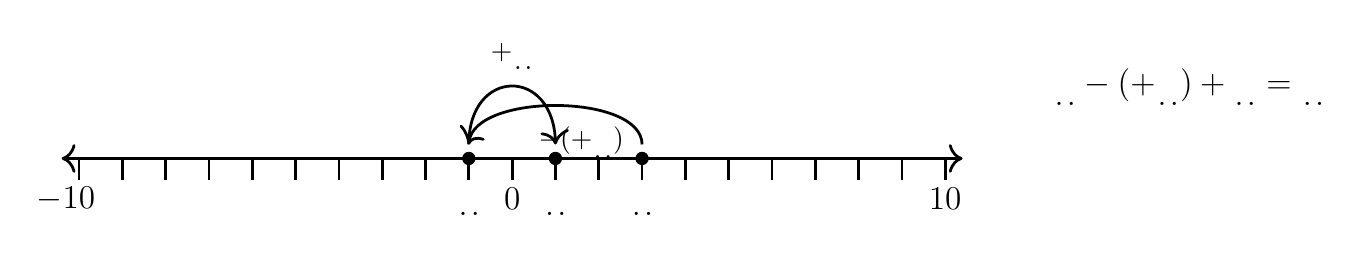
\begin{tikzpicture}[scale=0.55, baseline={([yshift=-1pt]current bounding box.north)}]
    % axis, arrow style to-to
    \draw[{To[scale=1.3]}-{To[scale=1.3]}, line width=1pt] (-10.4, 0) -- (10.4, 0);
    % tick marks
    \foreach \x in {-10,-9,...,10}
        \draw[shift={(\x,0)},color=black, line width=1pt] (0pt,-14pt) -- (0pt,0pt);
    % numbers along each axis
    \foreach \x in {-10}
        \draw[shift={(\x -0.3,-0.8)},color=black] node[font=\large,text height=12pt] {$\x$};
    \foreach \x in {0,10}
        \draw[shift={(\x,-0.8)},color=black] node[font=\large,text height=12pt] {$\x$};
    % numbers for dots
    \draw[shift={(3,-0.8)},color=black] node[font=\large,text height=12pt] {$\qgap$};
    \draw[shift={(-1,-0.8)},color=black] node[font=\large,text height=12pt] {$\qgap$};
    \draw[shift={(1,-0.8)},color=black] node[font=\large,text height=12pt] {$\qgap$};
    % dots
    \filldraw[black] (3,0) circle (4pt) node[above,yshift=-2pt] (a) {};
    \filldraw[black] (-1,0) circle (4pt) node[above,yshift=-2pt] (m) {};
    \filldraw[black] (1,0) circle (4pt) node[above,yshift=-2pt] (b) {};

    % first arrow (label below to left)
    \draw[-{To[scale=1.3, bend]}, line width=1pt, color=black] (a.north)
        .. controls +(north:\jumpheight mm) and +(north:\jumpheight mm) ..
        node[above=-9pt, xshift=-22pt, font=\normalsize, text height=8pt, pos=0] {$-(+\qgap)$} (m.north);

    % second arrow (label above)
    \draw[-{To[scale=1.3, bend]}, line width=1pt, color=black] (m.north)
        .. controls +(north:\jumpheighthigh mm) and +(north:\jumpheighthigh mm) ..
        node[above=2pt, font=\normalsize, text height=8pt] {$+\qgap$} (b.north);

    % equation at right end
    \node [font=\large, anchor=east] at (19,1.65) {$\qgap-(+\qgap)+\qgap = \qgap$};
\end{tikzpicture}
\end{equation}
\vspace{-2pt}\pagebreak ~ \newline ~ \newline\begin{equation}
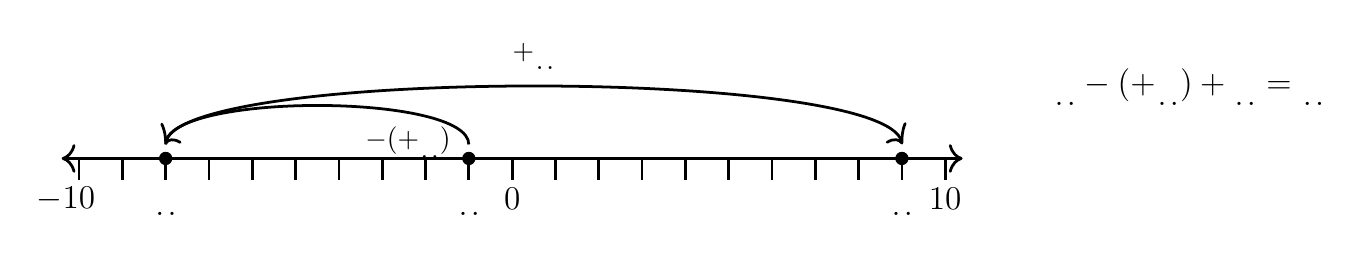
\begin{tikzpicture}[scale=0.55, baseline={([yshift=-1pt]current bounding box.north)}]
    % axis, arrow style to-to
    \draw[{To[scale=1.3]}-{To[scale=1.3]}, line width=1pt] (-10.4, 0) -- (10.4, 0);
    % tick marks
    \foreach \x in {-10,-9,...,10}
        \draw[shift={(\x,0)},color=black, line width=1pt] (0pt,-14pt) -- (0pt,0pt);
    % numbers along each axis
    \foreach \x in {-10}
        \draw[shift={(\x -0.3,-0.8)},color=black] node[font=\large,text height=12pt] {$\x$};
    \foreach \x in {0,10}
        \draw[shift={(\x,-0.8)},color=black] node[font=\large,text height=12pt] {$\x$};
    % numbers for dots
    \draw[shift={(-1,-0.8)},color=black] node[font=\large,text height=12pt] {$\qgap$};
    \draw[shift={(-8,-0.8)},color=black] node[font=\large,text height=12pt] {$\qgap$};
    \draw[shift={(9,-0.8)},color=black] node[font=\large,text height=12pt] {$\qgap$};
    % dots
    \filldraw[black] (-1,0) circle (4pt) node[above,yshift=-2pt] (a) {};
    \filldraw[black] (-8,0) circle (4pt) node[above,yshift=-2pt] (m) {};
    \filldraw[black] (9,0) circle (4pt) node[above,yshift=-2pt] (b) {};

    % first arrow (label below to left)
    \draw[-{To[scale=1.3, bend]}, line width=1pt, color=black] (a.north)
        .. controls +(north:\jumpheight mm) and +(north:\jumpheight mm) ..
        node[above=-9pt, xshift=-22pt, font=\normalsize, text height=8pt, pos=0] {$-(+\qgap)$} (m.north);

    % second arrow (label above)
    \draw[-{To[scale=1.3, bend]}, line width=1pt, color=black] (m.north)
        .. controls +(north:\jumpheighthigh mm) and +(north:\jumpheighthigh mm) ..
        node[above=2pt, font=\normalsize, text height=8pt] {$+\qgap$} (b.north);

    % equation at right end
    \node [font=\large, anchor=east] at (19,1.65) {$\qgap-(+\qgap)+\qgap = \qgap$};
\end{tikzpicture}
\end{equation}
\vspace{-2pt}
\end{document}

